
\graphicspath{{part_6/figures}{part_6/figures/}}

\section*{Terminology}
%====================
%
\begin{tabular}{ll}
$C_\Omega$ & Poincar\'e's constant (depending on $\Omega$) \\
$f$ & Source heat term of the heat equation \\
$g = -\frac{\partial u_q}{\partial t}(.;\bxi(t))$ & Source term the the equation in $\psi$\\
$K$ & Reduced-order truncation rank (low-order dimension) \\
$\kappa(.)$ & (space-varying) conductivity coefficient \\
$\kappa_m$ & Minimal conductivity coefficient \\
$K$ & Truncation rank for the reduced-order space \\
$L$ & Length of the spatial interval \\
$M$ & Number of control modes \\
$\psi=\psi(.,t)$ & such that $u(.,t) = u^\infty(.)+u_q(.,t) + \psi(.,t)$ \\
$\tilde \psi$ & reduced-order model for $\psi$ \\
$r_\xi(v)$ & Residual of the approximate heat solution $\tilde \psi$ against $v$ \\
$\Omega=(0,L)$ & Spatial domain \\
$\rho$ & Tolerance radius for the distance between $u$ and $u^\infty$ \\
$R_\xi$ & Recurrence set for the $\bxi$ variable \\
$\Sigma^\tau$ & Space of admissible switch control sequences \\
$U$ & the set of switched modes \\
$\tau$ & Switching sampling time \\
$t$ & Time variable \\
$u=u(x,t)$ & Solution of the controlled heat problem \\
$\tilde u=\tilde u(x,t)$ & Appxoximate reduced-order solution of the heat problem \\
$u^\infty(.)$ & ``Objective'' heat function \\
$u_q(.,t)$ & Solution of the quasistatic heat problem at time $t$ \\
$V=H^1_0(\Omega)$ & Sobolev space \\
$x$ & Space variable \\
$\bxi(t)=(\xi_1(t),\xi_2(t))^T$ & Vector of boundary control values \\
$\xi_1^\infty$ & $=u^\infty(0)$ \\
$\xi_2^\infty$ & =$u^\infty(L)$ \\
$\bxi^\infty$ & $=(\xi_1^\infty,\xi_2^\infty)^T$  \\
$W^K=\mathop{span}(\varphi^1,...,\varphi^K)$ & Reduced-order linear space, $W^K\subset V$
\end{tabular}
%
\section{Introduction}

In the previous chapter, we managed to synthesize reduced order controllers
for high dimensional ODEs, obtained from the discretization of PDEs.
We now want to use this kind of techniques, for results on the PDE problem.
A first possibility would have been to use error estimations of the 
discretization techniques employed, such as the ZZ estimators \cite{zienkiewicz1987simple}
for finite element methods. 
However, such a procedure uses an intermediate step (discretization) inevitably adding 
what we could call modeling error. 
In this chapter, we aim at keeping a PDE formulation undiscretized, and by properly 
transforming the problem, synthesizing low order controllers.
We first provide some of the developments made to obtain such results, and show the 
underlying difficulties. We first tried to use simple projection methods, such as 
spectral methods, associated to the Empirical Interpolation Method (EIM) \cite{maday2007general}.
The EIM is a recent algorithm which provides the best sets of points for Lagrangian interpolation,
which permits to efficiently represent complex functions with few generating functions. 
It has been derived for many efficient reduced basis methods.
The EIM was one of our first choices for guaranteed control of PDEs since it comes with
an $L^\infty$ error bound, and it seemed to be a natural way of obtaining 
continuous equivalents of Chapter \ref{chap:3}.
It revealed more complicated than expected to derive an $L^\infty$
guaranteed control, but we hope that these results might be of interest for 
future works.
After a long time struggling on $L^\infty$ bounds, we finally 
came to a change of topology for our reduced models, in order to 
develop $L^2$ guaranteed controls. As a matter of fact,
$L^2$ error bounds are actually much more classical 
in the field of structural mechanics, particularly when it comes 
to reduced order modeling. 
We thus present a second approach, aimed at synthesizing $L^2$
guaranteed controls.
The goal is now to use Galerkin methods for model order reduction, which is much more 
general than the balanced truncation or spectral methods, and allows to adapt the reduction 
technique to PDE problem. A second objective is to get an $L^2$ error estimation directly
for the PDE problem, and not a discretized version. 
In the following, we present our approaches on a given coupled ODE-PDE problem, for which the ODE is 
controlled.

% At first, we looked for $L^\infty$ error bounds, which seemed to be natural since 
% it provides guarantees available for the whole domain of the PDE. We first aimed 
% at adapting the Empirical Interpolation Method \cite{EIM,???}.



%
%{\color{red} BLA}
%%
%$M$ modes.
%
%Definition of the space $\Sigma^\tau$ of admissible sequences of switched control $\sigma(.)$
%of length less or equal to $P$~:
%

%
%
\section{Setting of the problem}
%==============================

Let $L>0$, let $\Omega=(0,L)$ be the domain of definition of the PDE. \medskip
Let $\kappa\in L^\infty(0,L)$, and suppose there exists two constants $\kappa_m$ and $\kappa_M$,
$0<\kappa_m\leq \kappa_M$ such that
\[
\kappa_m \leq \kappa(x) \leq \kappa_M \mbox{ for a.e. } x\mbox{ in } [0,L]. 
\]
The space of admissible switch control sequences is
%
\begin{equation}
\Sigma^\tau = \left\{ \sigma:[0,+\infty[ \rightarrow \{1,...,M\}, 
\sigma|_{[q\tau,(q+1)\tau[}(t)\in U\ \forall q\in \mathbb{N} \right\}.
\end{equation}
%
In this chapter, we consider the one-dimensional boundary switched control heat problem:
find a piecewise constant sequence $\sigma(.)\in \Sigma^r$, such that the vector-valued state
$\bxi(.)\in[\mathscr{C}^0_b(0,\infty)]^2$ and the function $u\in L^2(0,\infty; H^1(\Omega))$
solutions of the problem
%
\begin{eqnarray}
&& \frac{d\bxi}{dt} = A_\sigma \bxi + \bbb_\sigma, \quad t>0, \label{eq:2} \\ [1.1ex]
&& \bxi(0) = \bxi^0, \label{eq:3} \\ [1.1ex]
&& \frac{\partial u}{\partial t} - \nabla\cdot(\kappa(.)\nabla u) = f \quad 
\mbox{ in } \Omega\times (0,+\infty), \\ [1.1ex]
&& u(0,t) = \xi_1(t), \quad \mbox{ for all } t>0, \\ [1.1ex]
&& u(L,t) = \xi_2(t), \quad \mbox{ for all } t>0, \\ [1.1ex]
&& u(.,t=0) = u^0 \label{eq:7}
\end{eqnarray}
%
verify, for any initial conditions $\bxi_0$ and $u_0$, the stability constraints
%
\begin{equation}
\left\{\begin{array}{l}
\bxi(t) \in R_\xi \quad \mbox{ for all } t>0, \\ [1.1ex]
\| u(.,t)-u^{\infty}(.)\|_{L^2(\Omega)} \leq \rho \quad \mbox{ for all } t>0. 
\end{array}\right.
%
\label{eq:requirements}
%
\end{equation}
%
Thus the expected recurrence set for the global state $(\bxi(t),u(.,t))$
is the product set 
$R_\xi\times B(u^{\infty},\rho;\, L^2(\Omega))\subset \mathbb{R}^2\times L^2(\Omega)$. 
The sequence $\sigma(.)$ will depend on the state of the system itself in order to 
enforce stability in the product recurrence set.
The control problem is formalized as follows:
%
\begin{problem}[ODE-PDE stability control problem]
 Let us consider the equation system \eqref{eq:2}-\eqref{eq:7}.
 Given a set $R_\xi$, a tolerance $\rho$ and an objective state $u^\infty(\cdot)$,
 find a rule $\sigma((\bxi,u)) \in \Sigma^\tau$ such that, 
 for all $t >0$ and for all $(\bxi (0),v(x,0))\in R_\xi\times B(u^{\infty},\rho;\, L^2(\Omega))$,
 we have $(\bxi(t),u(.,t)) \in  R_\xi\times B(u^{\infty},\rho;\, L^2(\Omega))$.
 \label{prob:control} 
\end{problem}
We can also consider the reachability problem:
\begin{problem}[ODE-PDE reachability control problem]
 Let us consider the equation system \eqref{eq:2}-\eqref{eq:7}.
 Given two set $R_\xi$ and $R'_\xi$ with $R'_\xi \subset R_\xi$, two tolerances $\rho$ and $\rho'$
 with $\rho' < \rho$,
 and an objective state $u^\infty(\cdot)$,
 find a rule $\sigma((\bxi,u)) \in \Sigma^\tau$ such that, 
  for all $(\bxi (0),v(x,0))\in R_\xi\times B(u^{\infty},\rho;\, L^2(\Omega))$,
 there exists a time $t'> 0$ such that for all $t > t'$ we have 
 $(\bxi(t),u(.,t)) \in  R'_\xi\times B(u^{\infty},\rho';\, L^2(\Omega))$.
 \label{prob:control2} 
\end{problem}

\section{Spectral decomposition and EIM}

We now present our first approach, based on a spectral decomposition 
associated to the EIM \cite{maday2007general}.

\subsection{Problem statement}

Let us first consider a slightly simpler (linear) problem, on which 
we already see the complexity of the problem.

We wish to consider the equation system (\ref{eq:ODE}-\ref{eq:PDE}-\ref{eq:BC1}-\ref{eq:BC2}) 
given by:
\begin{eqnarray}
&& \frac{d\bxi}{dt} = A_\sigma \bxi + \bbb_\sigma, \quad t>0, \label{eq:ODE} \\ [1.1ex]
% && \bxi(0) = \bxi^0, \label{eq:3} \\ [1.1ex]
&& \frac{\partial u}{\partial t} - \frac{1}{\alpha}\nabla\cdot(\nabla u) = f \quad 
\mbox{ in } \Omega\times (0,+\infty), \label{eq:PDE}\\ [1.1ex]
&& u(0,t) = \xi_1(t), \quad \mbox{ for all } t>0, \label{eq:BC1}\\ [1.1ex]
&& u(L,t) = \xi_2(t), \quad \mbox{ for all } t>0, \label{eq:BC2}\\ [1.1ex]
% && u(.,t=0) = u^0 
\end{eqnarray}

% \begin{itemize}
%  \item an ODE of dimension 2 ($\bx \in \mathbb{R}^2$):
% \begin{eqnarray}
%  && \dot{\bm{a}} = \bm{b}_u
%  \label{eq:ODE}
% \end{eqnarray}
% 
% \item a parabolic PDE:
% \begin{equation}
%  \alpha \dfrac{\partial v}{ \partial t} -  \dfrac{\partial^2 v}{ \partial x^2} = 0 \quad\mbox{ in } \Omega 
% \label{eq:PDE}
%  \end{equation}
% with Dirichlet boundary conditions 
% \begin{eqnarray}
% && v(0,t) = a_1(t) \label{eq:BC1} \\
% && v(1,t) = a_2(t)
% \label{eq:BC2}
% \end{eqnarray}
% 
% \end{itemize}

% The state of the system is given by $(\bxi,u)$.
% The ODE is controlled by a control input $u$ belonging to a finite set $U = \{1,2,3,4\}$.
% System (\ref{eq:ODE}-\ref{eq:PDE}-\ref{eq:BC1}-\ref{eq:BC2}) is thus a switched controlled system.
% We suppose that switchings occur periodically, every $\tau$ seconds.

We suppose that we have four switched modes: 

$\bm{b}_1 = \left( \begin{array}{c}1\\1\end{array} \right)$ , $\bm{b}_2 = \left( \begin{array}{c}-1\\-1\end{array} \right)$,
$\bm{b}_3 = \left( \begin{array}{c}-1\\1\end{array} \right)$, $\bm{b}_4=\left( \begin{array}{c}1\\-1\end{array} \right)$

% The objective is to compute a control rule $\sigma(t)$ so that the state $u(x,t)$ of the PDE
% is as close as possible to $0$ for $x \in \Omega$ and for all $t>0$. We would like 
% to synthesize a state-dependent switching rule, i.e. $\sigma(t) = \tilde sigma((\ba(t),v(t)))$.
% The problem is formalized as follows:




% 
% In order to stabilize the state of the PDE around $0$, we can for example
% set $R = [-1,1]^2 \times [-1,1] $ and $R_t = [-0.2,0.2]^2 \times [-0.2,0.2]$, so that
% for any $v(x,0)$ belonging to $[-1,1]$ for $x \in \Omega$, and 
% $\ba(0)$ belonging to $[-1,1]^2$, $v(x,t)$ reaches and returns infinitely 
% often in $[-0.2,0.2]$ for $x \in \Omega$, and $\ba(t)$ reaches and returns
% infinitely often in $[-0.2,0.2]^2 $ (this is a recurrence property,
% a.k.a. stability is the sense of MINIMATOR).

In order to apply a symbolic (guaranteed) control synthesis method, we need to rewrite the system
under the form of an ODE of lowest possible dimension $m$:
\begin{equation}
 \dot \by = A \by + \bm{d}_\sigma
 \label{eq:symbolic}
\end{equation}
where $\by \in \mathbb{R}^m$, $A \in \mathbb{R}^{m\times m}$, $\bm{d}_\sigma \in \mathbb{R}^m$.

For this purpose, we will first write a low dimensional equation with a 
spectral model reduction.
% \subsection{Symbolic control}
% Control synthesis by state-space decomposition (MINIMATOR).
% Available for systems of the form (\ref{eq:symbolic}).
% 
% 
% Permits to send a set of states $R$ (a box of $\mathbb{R}^m$) to
% a target set $R_{t}$ (a box of $\mathbb{R}^m$).
% 
% The state of a PDE is of infinite dimension. Supposing that a finite element discretization is used, 
% the state dimension is finite, but much higher than what can be handled by guaranteed symbolic 
% methods. We thus need thus need  a Model Order Reduction in order to reduce the state
% dimension.


\subsection{Spectral Model Reduction}
\label{sec:ROM}

We wish to approximate the state $u(x,t)$ of the PDE by a 
state $\tilde u (x,t)$ as close as possible to $u(x,t)$, 
but which can be computed much more easily than by solving the PDE (e.g. with a finite element
method). A natural way of computing an approximate solution 
of (\ref{eq:PDE}) is using a modal (spectral) decomposition [ref?].
An accurate approximate solution of (\ref{eq:PDE}) can be obtained with few 
eigen modes when the boundary conditions are homogeneous. This is why we 
use here a reduced model made of a modal decomposition with a lifting:
\begin{equation}
\tilde u(x,t) =  \xi_1(t)(1-x) + \xi_2(t)x + \sum_{i = 1}^N \beta_i (t) \varphi_i (x)
\label{eq:ROM}
\end{equation}
where the $\beta_i$ are the time coefficients associated to the space functions $\varphi_i$,
which are precomputed (the computation of the $\varphi_i$ is detailed in
the following). 

Let us explain why the lifting is interesting. 
If we write $\tilde u(x,t) =  \xi_1(t)(1-x) + \xi_2(t)x + w(x,t)$ and inject it in (\ref{eq:PDE},\ref{eq:BC1},\ref{eq:BC2}),
we have:


\begin{align*}
& \alpha \dfrac{\partial \tilde u}{ \partial t} -  \dfrac{\partial^2 \tilde u}{ \partial x^2} = 0 \quad\mbox{ in } \Omega \\
& \tilde u (0,t) = \xi_1(t) \\
& \tilde u (1,t) = \xi_2(t)
\end{align*}


\begin{align*} 
& \alpha \left( \dot \xi_1(t)(1-x) + \dot \xi_2(t)x + \dfrac{\partial w}{ \partial t} \right) -  \dfrac{\partial^2 w}{ \partial x^2} = 0 \quad\mbox{ in } \Omega \\
& w(0,t) + \xi_1(t) = \xi_1(t) \\
& w (1,t) + \xi_2(t) = \xi_2(t)
\end{align*}

\begin{align*}
& \alpha \dfrac{\partial w}{ \partial t}  -  \dfrac{\partial^2 w}{ \partial x^2} = -\alpha ( \dot \xi_1(t)(1-x) + \dot \xi_2(t)x) \quad\mbox{ in } \Omega \\
& w(0,t) = 0 \\
& w(1,t) = 0
\end{align*}


The lifting $\xi_1(t)(1-x) + \xi_2(t)x$ permits to obtain homogeneous boundary conditions
for $w$.
The associated eigenvalue problem $\phi'' = \mu \phi$ with homogeneous boundary 
conditions leads to eigenmodes (see \cite{cain2005separation}):
\begin{equation}
\varphi_i(x) = \sqrt{2} \sin{(i \pi x)}
\label{eq:modes}
\end{equation}
Note that the eigenmodes $\varphi_i$ have been normalized w.r.t.
the scalar product $\langle \cdot , \cdot \rangle_\Omega$.
A solution for $w$ can then be decomposed on the basis of 
the eigenmodes $w(x,t) = \sum_{i=1}^\infty \beta_i(t)\varphi_i(x)$.
Having written $w$ under this last form,
an exact solution for equations (\ref{eq:PDE},\ref{eq:BC1},\ref{eq:BC2}) can be found as
\begin{equation}
\alpha \dfrac{\partial w}{ \partial t}  -  \dfrac{\partial^2 w}{ \partial x^2} = \sum_{i=0}^\infty \langle -\alpha ( \dot \xi_1(t)(1-x) + \dot \xi_2(t)x) , \varphi_i \rangle_\Omega \varphi_i
\end{equation}
% 
% Using a modal decomposition means that 
% the functions $\varphi_i$ are computed as the eigenmodes of this last equation system
% (\ref{eq:PDE_homo1} - \ref{eq:PDE_homo3}), see \cite{cain2005separation} for details of the computation (NB: we normalize it w.r.t. 
% the scalar product $\langle \cdot , \cdot \rangle_\Omega$).
% To obtain an exact solution, we should make $N$ tend to infinity, but one can 
% often use only few functions to accurately represent the solution. 
% We have: 


Instead, we will look for an approximate solution by truncating the sum at
an order $N$.
Let us now find $\tilde u(x,t)$ of the form (\ref{eq:ROM}), solution 
of the equation system (\ref{eq:PDE}) with boundary conditions (\ref{eq:BC1}-\ref{eq:BC2}).
We have:

$$ \alpha \dfrac{\partial \tilde u}{ \partial t} -  \dfrac{\partial^2 \tilde u}{ \partial x^2} = 0 \quad\mbox{ in } \Omega $$

$$ \alpha \dfrac{\partial \tilde u}{ \partial t} w -  \dfrac{\partial^2 \tilde u}{ \partial x^2}w = 0  \quad\mbox{ in } \Omega \quad \forall w \in H^1_0(\Omega)$$

Writing the weak form formulation and using an integration by parts, we obtain:

$$ \alpha \dfrac{d}{dt} \int_\Omega \tilde u w dx + \int_\Omega \dfrac{\partial \tilde u}{\partial x} \dfrac{\partial w}{\partial x} dx = 0 \quad \forall w \in H_0^1(\Omega) $$

This is true for all $w \in H_0^1(\Omega)$, we can thus write:

$$\displaystyle{ \alpha \dfrac{d}{dt} \int_\Omega \tilde u w dx + \int_\Omega \dfrac{\partial \tilde u}{\partial x} \dfrac{\partial w}{\partial x} dx =0, \quad \forall w \in W^k = \text{Vect}(\varphi_k)}$$

Which leads to:

 \begin{multline*}
 \displaystyle{ \alpha \int_\Omega ((1-x) \dot \xi_1 + x \dot \xi_2) \varphi_k dx + \int_\Omega ((1-x) \xi_1 + x \xi_2) \dfrac{\partial \varphi_k}{\partial x} dx } \\ 
 \displaystyle{+ \alpha \sum_{i=1}^N \dot \beta_i \int_\Omega \varphi_i \varphi_k dx + \sum_{i=1}^N \beta_i \int_\Omega \dfrac{ \partial \varphi_i}{\partial x} \dfrac{ \partial \varphi_k}{\partial x} dx = 0, \quad \forall k = 1,\dots,N}
 \end{multline*}

\vspace{1em}

The second term being equal to zero, we then have a low dimensional equation:
\begin{equation}
 \alpha C_r \dot{\bm{\beta}} + K_r \bm{\beta} = - \alpha \bm{F_r}(\dot{\bxi},t)
 \label{eq:red}
\end{equation}

with $\bm{\beta}$ the vector composed of the $\beta_i$, which we call 
the reduced state, $C_{r,ij} = \int_\Omega  \varphi_i \varphi_j dx$, $K_{r,ij} = \int_\Omega  \dfrac{ \partial \varphi_i}{\partial x} \dfrac{ \partial \varphi_j}{\partial x} dx$
and ${F_{r,i}}(\dot{\bxi},t) = \int_\Omega ((1-x) \dot \xi_1 + x \dot \xi_2) \varphi_i dx$.
Note here that matrices $C_r$ and $K_r$ are diagonal, because functions $\varphi_i$
are orthogonal. This is one of the main advantages
in using such a modal decomposition: an accurate approximate solution
can be computed in a very cheap way.

Solving the equation system (\ref{eq:ODE}-\ref{eq:PDE}-\ref{eq:BC1}-\ref{eq:BC2})
with the reduced order solution (\ref{eq:ROM}) then leads to solving
the reduced system:


\begin{equation}
\label{eq:sys_red}
  \left( \begin{array}{c}
  \dot{\bxi}(t) \\ \dot{\bm{\beta}}(t)
 \end{array} \right) = \left( \begin{matrix} 0 & 0 \\ 0 & 1/\alpha C_r^{-1} K_r \end{matrix} \right)\left( \begin{array}{c}
   \bxi(t) \\ \bm{\beta}(t)
 \end{array} \right) + \begin{pmatrix}
                        \bm{b}_u(t) \\ -C_r^{-1} \bm{F_r}(\bm{b}_u(t),t)
                       \end{pmatrix}
\end{equation}



However, although the lifting $\xi_1(t)(1-x) + \xi_2(t)x$ permits to construct an accurate reduced model 
with few functions $\varphi_i$, it raises a new problem:
the coefficients $\beta_i$ have no physical meaning. 
It is thus not trivial to infer a reduced objective (a box, or an objective set)
for the reduced state $\bm{\beta}$. In other words, we do not know 
where the $\beta_i$ should stabilize to obtain a PDE state as close to zero as we want. 

In order to give a physical meaning to the reduced state, and infer an initial and objective
box the reduced state variable, we build a reduced model with slightly 
different basis functions:

\begin{equation}
\tilde u(x,t) =  \xi_1(t)(1-x) + \xi_2(t)x + \sum_{i = 1}^N \gamma_i (t) \psi_i (x)
\end{equation}

where functions $\psi_i$ interpolate $N$ points $x_1, \dots, x_N$  of the PDE domain, i.e.:

\begin{equation}
 \psi_i (x_j) = \delta_{ij} \quad \forall i \in \{1,\dots,N \}.
 \label{eq:interp}
 \end{equation}
Here, $\delta_{ij}$ denotes the Kronecker symbol.
The functions $\psi_i$, as well as the interpolated points $x_i$, are 
computed with the EIM \cite{maday2007general}. The use of the EIM is particularly 
opportune since it permits to establish an $L^\infty$ error bound which 
allows to compute a guaranteed control (see Section \ref{sec:bound}).
Furthermore, the interpolated points are optimal and lead to the lowest possible error bound.

The algorithm for computing the interpolation points is the following:

Let $x_1 = \arg \max_{x \in \Omega} | \varphi_1 (x)|$.

% Functions $\{ \psi_1, \dots, \psi_N \}$ and 
Interpolation points $\{x_1, \dots x_N \}$
are then constructed by induction on $M\leq N$ as follows.
For all $i$, $1\leq i \leq M-1$, solve $\varphi_M (x_i) = \sum_{j = 1}^{M-1} h_{ij}^{M-1}  \varphi_j (x_i)$
for $h_{ij}^{M-1}$,
and set $x_M = \arg \max_{x \in \Omega} | \varphi_M (x) - \sum_{j=1}^{M-1} h_{ij}^{M-1} \varphi_j(x) |$.
In the EIM terminology, $\sum_{j=1}^{M-1} h_{ij}^{M-1} \varphi_j(\cdot)$ is denoted as the 
interpolant $\mathcal{I}_{M-1}[ \varphi_M (\cdot) ]$ since it interpolates exactly $\varphi_M (\cdot)$
in $x_1,\dots, x_{M-1}$. 

Functions $\psi_i$ are then computed as linear combinations of the functions $\varphi_i$
as follows. For all $1\leq i \leq N$, solve
$\sum_{j=1}^N \varphi_j(x_i) h_{ij}^N = \delta_{ij}$ for $h_{ij}^N$.
Then set $\psi_i = \sum_{j = 1}^ N h_{ij}^N \varphi_j$ so
that functions $\psi_i$ do verify (\ref{eq:interp}).
In the following, for any $u \in H^1 ( \Omega)$, we will denote by $\mathcal{I}_N [u(\cdot)]$ the 
interpolation of order $N$ of $u(\cdot)$, i.e. $\mathcal{I}_N [u(\cdot)] = \sum_{i=1}^N u(x_i) \sum_{j = 1}^ N h_{ij}^N \varphi_j(\cdot)$.

The reduced system is then computed just as system (\ref{eq:sys_red}) but with functions
$\psi_i$ instead of $\varphi_i$, this leads to:
\begin{equation}
  \left( \begin{array}{c}
  \dot{\bxi}(t) \\ \dot{\bm{\gamma}}(t)
 \end{array} \right) = \left( \begin{matrix} 0 & 0 \\ 0 & 1/\alpha C_r'^{-1} K_r' \end{matrix} \right)\left( \begin{array}{c}
   \bxi(t) \\ \bm{\gamma}(t)
 \end{array} \right) + \begin{pmatrix}
                        \bm{b}_u(t) \\ -C_r^{-1} \bm{F_r'}(\bm{b}_u(t),t)
                       \end{pmatrix}
\label{eq:red2}                       
\end{equation}
with $\bm{\gamma}$ the vector composed of the $\gamma_i$, which we call 
the reduced state, $C'_{r,ij} = \int_\Omega  \psi_i \psi_j dx$, $K'_{r,ij} = \int_\Omega  \dfrac{ \partial \psi_i}{\partial x} \dfrac{ \partial \psi_j}{\partial x} dx$
and ${F'_{r,i}}(\dot{\bxi},t) = \int_\Omega ((1-x) \dot \xi_1 + x \dot \xi_2) \psi_i dx$.
Note that here, matrices $C'_{r}$ and $K'_{r}$ are no longer diagonal, which results 
in slightly higher computation costs, but since the dimension of those matrices
must be low, this is not prohibitive. 

% The only problem which could result in using such interpolating
% reduced functions is that we may obtain an ill-conditioned reduced system (\ref{eq:red2}) 
% (particularly if the interpolated points are chosen close to each other). (est-ce que c'est toujours vrai???)

% In the following, we use arbitrary interpolation points, but an EIM approach [ref Maday] could be 
% used to select the best interpolation points.

The main interest in using interpolating functions is 
that the variables $\gamma_i$ have now a physical meaning: $\gamma_i(t)$ 
is equal to the value the temperature field (without lifting) in $x_i$ at time $t$.

We have:
\begin{equation}
\tilde u(x_i,t) =  \xi_1(t)(1-x_i) + \xi_2(t)x_i +  \gamma_i (t), \quad \forall i \in \{1,\dots, N\}
\end{equation}

If we want $u(x_i,t)$ to stay in a box $[u_i^{min},u_i^{max}]$, then 
we have to ensure that $\xi_1,\xi_2 \in [u_i^{min}/2,u_i^{max}/2]$, 
and $\gamma_i \in [u_i^{min}/2,u_i^{max}/2]$ (note that other combinations are possible).

\subsection{Error bounding}
\label{sec:bound}

With the above developments, we can ensure that $\tilde u(x_i,t)$ reaches infinitely often the box $[u_{min},u_{max}]$
with symbolic methods thanks to equation \eqref{eq:red2}.
In order to provide a guaranteed controller,
we still need to bound the error between the reduced order and the full
order system.
The minimal result required to ensure 
recurrence is to bound: $\vert \tilde u (x_i,t) - u(x_i,t) \vert$ for all $t >0$.
Or, more precisely, for a pattern of length $k$, compute a bound $\varepsilon_1 (k)$ such that:
\begin{equation}
 | u(x_i,t_0 + k \tau) - \gamma_i(t_0 + k \tau) | \leq \varepsilon_1(k) \quad \forall i = 1, \dots,N
\end{equation}

But in order to ensure that the whole state $u(x,t)$ stays in $[u_{min},u_{max}]$, 
we also need to bound $\vert \tilde u (x,t) - u(x,t) \vert$ for all $x \in \Omega$ and $t \geq 0$.
We thus need to obtain an $L^\infty$ bound. I.e., for all $k \geq 0$,
compute a bound $\varepsilon_2(k)$ such that:
\begin{equation}
 \| u(\cdot,t_0 + k \tau) - \tilde u(\cdot,t_0 + k \tau) \|_{L^\infty(\Omega)} \leq \varepsilon_2(k) 
\end{equation}











As mentioned above, the EIM provides an $L^\infty$ error bound.
% W.I.P.
% 
% Let us introduce some notations:
% 
% \begin{definition}[$Post$ operator]
% Let $t_0 \in \mathbb{R}$. Suppose that a mode $u \in U$ is applied between times $t_0$ 
% and $t_0 + \tau$.
%  Let $\bxi_0 = \bxi (t_0) \in \mathbb{R}^2$ and $v_0 = v(\cdot,t_0) \in H^1(\Omega)$ with $v(0,t_0) = \xi_1(t_0)$
%  and $v(1,t_0) = \xi_2(t_0)$.
%  
%  We denote by $Post_u(\bxi_0,v_0)$ the solution $(\bxi (t_0 + \tau), v(\cdot,t_0+\tau))$ at time $t_0 + \tau$ of the equation system 
%  (\ref{eq:ODE},\ref{eq:PDE},\ref{eq:BC1},\ref{eq:BC2}) with initial conditions
%  $\bxi_0$ and $v_0$.
%  \end{definition}
% 
%  Similarly, let us define the post operator for the reduced system:
%  \begin{definition}[Reduced $Post$ operator]
% Let $t_0 \in \mathbb{R}$. Suppose that a mode $u \in U$ is applied between times $t_0$ 
% and $t_0 + \tau$.
%  Let $\bxi_0 = \bxi (t_0) \in \mathbb{R}^2$ and $\bm{\gamma}_0 = \bm{\gamma} (t_0) \in \mathbb{R}^N$.
%  
%  We denote by $Post_u(\bxi_0,\bm{\gamma}_0)$ the solution $(\bxi(t_0 + \tau),(\tilde v(x_i,t_0 + \tau))_{i=1,\dots,N}) = (\bxi(t_0 + \tau), \bm{\gamma}(t + \tau))$ at time $t_0 + \tau$ of the equation system 
%  (\ref{eq:red2}) with initial conditions
%  $\ba_0$ and $\bm{\gamma}_0$.
%  \end{definition}
%  
 For all $M \geq 0 $ and for all $v \in H^1 ( \Omega)$, let $\{ \phi_k \}_{k = 1,\dots,M+1}$ be
 the first $M+1$ basis functions returned by the EIM for $v$, we have the following error bound 
 for  the EIM interpolant of $v$:
% \begin{itemize} 
% 
% \item $L^\infty$ bound with EIM version 1:
%  
%  \begin{equation}
%   \| v - \mathcal{I}_M [v] \|_{L^\infty(\Omega)} \leq (1 + \Lambda_M) \inf_{v_M \in \text{span} \{ \psi_i (\cdot), 1 \leq i \leq M \} } \| v - v_M \|_{L^\infty(\Omega)}
%  \end{equation}
% 
%  
%  \item $L^\infty$ bound with EIM version 2:
%  
%   \begin{equation}
%   \| v - \mathcal{I}_M [v] \|_{L^\infty(\Omega)} \leq  c e^{-(\alpha - log(4))M}
%   \end{equation}
% 
%   
%   \item $L^\infty$ bound with EIM version 3: 
   \begin{equation}
   \label{eq:EIM_bound}
  \| v(\cdot) - \mathcal{I}_M [v(\cdot)] \|_{L^\infty(\Omega)} \leq  \| \phi_{M+1}(\cdot) - \mathcal{I}_{M} [\phi_{M+1}(\cdot)] \|_{L^\infty(\Omega)}
  \end{equation} 
%   
%   
%  \end{itemize}


 
 
 



Let us suppose $\mathcal{I}_N $ has been computed as in Section \ref{sec:ROM}.
We have, for all $x \in \Omega$ and for all $t>0$:
\begin{equation}
 |v(x,t) - v_N(x,t) | \leq | v(x,t) - \mathcal{I}_N [v (\cdot,t)](x,t) | + |\mathcal{I}_N [v (\cdot,t)](x,t) - v_N(x,t) | 
\end{equation}
The first right-hand term $ | v(x,t) - \mathcal{I}_N [v (\cdot,t)](x,t) |$
can be bounded by the EIM bound (\ref{eq:EIM_bound}).
The second right-hand term $|\mathcal{I}_N [v (\cdot,t)](x,t) - v_N(x,t) |$ being
constructed with functions $\varphi_1,\dots,\varphi_N$,
it is equal, for all $t\geq0$ and $x \in \Omega$, to the analytical solution of the 
truncated projected solution:
$$\mathcal{I}_N [v (\cdot,t)] (x,t) - v_N(x,t) = \mathcal{I}_N [v (\cdot,t)](x,t) - \sum_{i=1}^N \beta_i(t) \varphi_i(x)$$

$$\mathcal{I}_N [v (\cdot,t)] (x,t) - v_N(x,t) = \mathcal{I}_N [v (\cdot,t)](x,t) - \sum_{i=1}^N \gamma_i(t) \psi_i(x)$$
% $$ \mathcal{I}_N [v (\cdot,t)](x,t) - v_N(x,t)  = v(x,t) - \sum_{i=1}^\infty \beta_i(t) \varphi_i(x) $$
We hoped to bound this term in the same fashion 
as \cite{eftang2010posteriori}, but it revealed more difficult than expected. 
The interpolation $\mathcal{I}_N [v (\cdot,t)](x,t)$ should in fact 
be computed for every time $t$, and bounding this 
for every time would be numerically irrelevant. 
As explained in \cite{eftang2010posteriori}, it is possible to bound such a
term when the state $v$ depends explicitly on a parameter, and for which 
the derivatives w.r.t the parameter can be computed. We hoped to evaluate this term by taking time
as a parameter, but this is actually not possible straightforwardly. We however
think that this term can be evaluated with further developments, using for example 
an EIM coupled with another model reduction such as the Proper Generalized 
Decomposition~\cite{chinesta2011short,chinesta2010recent}.

% 
% Let us recall that $v(x,t) = \xi_1(t) (1-x) + \xi_2(t) x + \sum_{i=1}^\infty \beta_i(t) \varphi_i(x)$.
% 
% 
% 
% 
% /!$\backslash$ Abus de notation: $R_t = R_t^2 \times R_t^N$
% 
% \begin{theorem}
%  Computing a decomposition with MINIMATOR such that, for all $(\bxi,\bm{\gamma})\in R$, and for a pattern $\pi$ of length $k$: 
% \begin{equation}
%  Post_\pi (\bxi,\bm{\gamma}) \in R_t^2/2 \times (R_t^N/2 - \varepsilon_1(k))
% \end{equation}
% ensures that we stabilize the system (\ref{eq:ODE}-\ref{eq:BC2}) with $v(x_i,k\tau) \in R_t$ for some multiples of $k$.
% \end{theorem}
% \textbf{Proof}
% 
% \begin{theorem}
%  Computing a decomposition with MINIMATOR such that, for all $(\bxi,\bm{\gamma})\in R$, and for a pattern $\pi$ of length $k$:
% \begin{equation}
%  Post_\pi (\bxi,\bm{\gamma}) \in R_t^2/2 \times (R_t^N/2 - \varepsilon_2(k))
% \end{equation}
% ensures that we stabilize the system (\ref{eq:ODE}-\ref{eq:BC2}) in $R_t$ (solves Problem \ref{prob:control}).
% \end{theorem}
% \textbf{Proof}
% 

\section{$L^2$ guaranteed control}

Having introduced our attempt of $L^\infty$ guaranteed control, we now present 
an $L^2$ approach closer to classical techniques used in the field of
structural mechanics. The reduced state we build will now be associated
with an $L^2$ distance instead of an Euclidean one, so that the sets (balls) 
defined on the reduced space have a meaning directly on the PDE state.
We now consider the original problem \eqref{eq:2}-\eqref{eq:7}.

\subsection{Transformation of the problem}
%----------------------------------------
%
Denoting by $u_q=u_q(.,t)$ the solution of the quasi-static problem at each time $t$:
%
\begin{eqnarray}
&&  - \nabla\cdot(\kappa(.)\nabla u_q) = f+\nabla\cdot(\kappa(.)\nabla u^\infty) \mbox{ in } \Omega, 
\label{eq:9}\\ [1.1ex]
&& u_q(0,t) = \xi_1(t)-\xi_1^\infty,  \\ [1.1ex]
&& u_q(L,t) = \xi_2(t)-\xi_2^\infty, 
\label{eq:11}
\end{eqnarray}
%
one can express the solution $u$ as the sum of $u^\infty$, $u_q$ and a function $\psi$, i.e.
%
\begin{equation}
u(.,t) = u^\infty(.) + u_q(.,t) + \psi(.,t)
\label{eq:decomp}
\end{equation}
%
where $\psi(.,t)$ is solution of the heat problem with homogeneous Dirichlet boundary conditions
%
\begin{eqnarray}
&& \frac{\partial \psi}{\partial t} - \nabla\cdot(\kappa(.)\nabla \psi) = g(.;\bxi(t))
\label{eqq:13}
\quad \mbox{ in } \Omega\times (0,+\infty) \\ [1.1ex]
&& \psi(0,t) = \psi(L,t) = 0, \quad t>0, \\ [1.1ex]
&& \psi(.,t=0) = \psi^0, \label{eqq:15}
\end{eqnarray}
%
with
\[
g(.;\xi(t)) = -\frac{\partial u_q}{\partial t}(.;\bxi(t)),
%+\nabla\cdot [\kappa(.)\nabla(u^\infty+u_q(.;\bxi(t)))],
\quad \psi^0 = u^0 -u^\infty - u_q(.,0).
\]
We thus consider the functional Sobolev space $V=H^1_0(\Omega)$.
The weak variational formulation of the problem~\eqref{eqq:13}-\eqref{eqq:15} is to find $\psi\in L^2(0,\infty;V)$, $\psi(.,t=0) = \psi^0$, solution of 
%
\begin{eqnarray}
&& (\frac{\partial \psi}{\partial t},v) + (\kappa(.)\nabla\psi,\nabla v)
= (g(.;\bxi(t)),v) \quad \forall v \in V. \label{eq:12}
\end{eqnarray}
The decomposition \eqref{eq:decomp} actually lets us study the different 
behaviors we observe in the equation: the quasi-static behavior, which is attained when 
the time step gets large; and the dynamic behavior, being observed mainly at the beginning 
of a switch. We also exhibit the objective state, and it will reveal the 
possible (attainable) target states.
%
\subsection{Stability requirements}
%--------------------------------
%
Because of~\eqref{eq:decomp}, the stability requirement
\begin{equation}
\| u(.,t)-u^{\infty}(.)\|_{L^2(\Omega)} \leq \rho \quad \mbox{ for all } t>0
\label{eq:stab1}
\end{equation}
in~\eqref{eq:requirements} can be equivalently expressed as
\[
\|u_q(.,t) + \psi(.,t)\|_{L^2(\Omega)} \leq \rho \quad \mbox{ for all } t>0.
\]
The solution $u_q$ itself can be decomposed as
\[
u_q(.,t) = \bar u(.) + w_q(.,t),
\]
where $\bar u$ is solution of the steady elliptic problem with homogeneous Dirichlet boundary conditions
\begin{eqnarray}
&& -\nabla\cdot(\kappa(.)\bar u) = 
f+\nabla\cdot(\kappa(.)\nabla u^\infty) \quad \mbox{ in } \Omega, \label{eq:18}\\
&& \bar u(0) = \bar u(L) = 0, \label{eq:19}
\end{eqnarray}
%
and $w_q$ is solution of the quasi-static problem at each time $t$:
%
\begin{eqnarray}
&&  - \nabla\cdot(\kappa(.)\nabla w_q) = 0 \mbox{ in } \Omega, 
\label{eq:20}\\ [1.1ex]
&& w_q(0,t) = \xi_1(t)-\xi_1^\infty, \quad \mbox{ for all } t>0, \\ [1.1ex]
&& w_q(L,t) = \xi_2(t)-\xi_2^\infty, \quad \mbox{ for all } t>0.
\label{eq:22}
\end{eqnarray}
%
The solution $\bar u$ is continuous with respect to the source term in~\eqref{eq:18} \cite{???}, i.e.
%
\begin{equation}
\|\bar u\|_V \leq C'\, \|f+\nabla\cdot(\kappa(.)\nabla u^\infty)\|_{L^2(\Omega)}.
\end{equation}
%
For the solution $w_q$ of~\eqref{eq:20}-\eqref{eq:22}, because of the maximum
principle, we have
%
\begin{equation}
\|w_q(.,t)\|_{L^\infty(\Omega)} = \max(|\xi_1(t)-\xi_1^\infty|,|\xi_2(t)-\xi_2^\infty|)
=\|\bxi(t)-\bxi^\infty\|_\infty.
\end{equation}
%
Thus, 
\begin{eqnarray*}
\|u_q(.,t)+\psi(.,t)\|_{L^2(\Omega)}&\leq& \|\bar u\|_{L^2(\Omega)} + \|w_q\|_{L^2(\Omega)} + \|\psi(.,t)\|_{L^2(\Omega)} \\
&\leq & \|\bar u\|_{L^2(\Omega)} + L \|w_q\|_{L^\infty}+ \|\psi(.,t)\|_{L^2(\Omega)}, 
\end{eqnarray*}
and finally
\begin{multline*}
\|u_q(.,t)+\psi(.,t)\|_{L^2(\Omega)} \leq  C \|f+\nabla\cdot(\kappa(.)\nabla u^\infty)\|_{L^2(\Omega)} \\ + L\,\|\bxi(t)-\bxi^\infty\|_\infty + \|\psi(.,t)\|_{L^2(\Omega)}
\end{multline*}


%
A sufficient condition to satisfy the stability constraint~\eqref{eq:stab1} is then to fulfill 
%
\begin{equation}
C \|f+\nabla\cdot(\kappa(.)\nabla u^\infty)\|_{L^2(\Omega)} + L\,\|\bxi(t)-\bxi^\infty\|_\infty + \|\psi(.,t)\|_{L^2(\Omega)} \leq \rho.
\label{eq:26}
\end{equation}
%
The solution~$\psi$ lives in an infinite-dimensional space, so that it is hard
or impossible to build a control synthesis based on a state-space decomposition. %that can fulfill~\eqref{eq:26}.  
In the sequel of the paper,
we will rather use a low-dimensional approximation $\tilde \psi$ (the reduced-order model of $\psi$) in the form
%
\begin{equation}
\tilde \psi(x,t) = \sum_{k=1}^K \tilde \beta_k(t) \varphi^k(x)
\end{equation}
%
with a reduced basis $\{\varphi^k\}_{k=1,...,K}$ assumed to be orthonormal in $L^2(\Omega)$.
In the sequel we will denote by $W^K$ the linear vector space of dimension $K$ spanned by the reduced basis $\{\varphi^k\}_k$:
\[
W^K = \mathop{span}\left(\varphi^1,...,\varphi^K\right).
\] 
Denoting by $\tilde \bbeta(t)=(\tilde\beta_1(t),...,\tilde\beta_K(t))^T$
the vector of coefficients, we then have
\[
\|\tilde \psi(.,t)\|_{L^2(\Omega)} = \|\tilde\bbeta(t)\|_{2,\mathbb{R}^K}.
\]
By the triangular inequality we can write
%
\begin{eqnarray}
\|\psi(.,t)\|_{L^2(\Omega)} &\leq& \|\psi(.,t)-\tilde\psi(.,t)\|_{L^2(\Omega)}
+\|\tilde \psi(.,t)\|_{L^2(\Omega)} \\ [1.1ex]
%
&\leq& \|\psi(.,t)-\tilde\psi(.,t)\|_{L^2(\Omega)} + \|\tilde\bbeta(t)\|_2.
\end{eqnarray}
%
Let us assume that we have the stability estimate for the reduced-order approximation: there exists a constant $\mu>0$
such that
%
\begin{equation}
% \boxed{
\|\psi(.,t)-\tilde\psi(.,t)\|_{L^2(\Omega)} \leq \mu\, \|\psi^0-\tilde\psi^0\|_{L^2(\Omega)}
\quad \forall t\in [0,\tau]
\label{eq:stab}
% }
\end{equation}
%
for any constant control mode $\sigma\in\{1,...,M\}$ (uniform stability with respect to the controls). 
This hypothesis can actually be verified with a proper construction
of the reduced basis. 
Then, a more restrictive sufficient condition to fulfill the stability constraint~\eqref{eq:stab1}
is to verify
%
\begin{multline}
% \boxed{
C \|f+\nabla\cdot(\kappa(.)\nabla u^\infty)\|_{L^2(\Omega)} + L\,\|\bxi(t)-\bxi^\infty\|_\infty 
\\ + \|\tilde\bbeta(t)\|_2
+ \mu\, \|\psi^0-\tilde \psi^0\|_{L^2(\Omega)}  \leq \rho.
% }
\label{eq:30}
\end{multline}
%
This equation is interesting since it enlightens the different controllable and uncontrollable 
terms. 


Let us denote by $\pi^K:V\rightarrow W^K$ the continuous linear orthogonal projection operator over
the low-order space $W^K$. Still by a triangular inequality, we have
\[
\|\psi^0-\tilde \psi^0\|_{L^2(\Omega)} \leq
\|\psi^0-\pi^K \psi^0\|_{L^2(\Omega)} + \|\pi^K\psi^0-\tilde \psi^0\|_{L^2(\Omega)},
\]
The projection $\pi^K \psi^0$ is given by
\[
\pi^K \psi^0 = \sum_{k=1}^K \beta_k^0\, \varphi^k, 
\]
with $\beta_k^0=(\psi^0,\varphi^k)_{L^2(\Omega)}$, $k=1,...,K$. By denoting 
$\bbeta^0=(\beta_1^0,...,\beta_K^0)$, we then have
\[
\|\psi^0-\tilde \psi^0\|_{L^2(\Omega)} \leq
\|\psi^0-\pi^K \psi^0\|_{L^2(\Omega)} + \|\bbeta^0-\tilde \bbeta^0\|_2,
\]
Another sufficient condition to fulfill the stability constraint~\eqref{eq:stab1}
is then
%
\begin{multline}
\small
% \boxed{
C\, \|f+\nabla\cdot(\kappa(.)\nabla u^\infty)\|_{L^2(\Omega)} + L\,\|\bxi(t)-\bxi^\infty\|_\infty + \|\tilde\bbeta(t)\|_2 \\
+ \mu\, \|\psi^0-\pi^K\psi^0\|_{L^2(\Omega)}+ \mu\, \|\bbeta^0-\tilde \bbeta^0\|_2 \leq \rho.
% }
\label{eq:31}
\normalsize
\end{multline}
%
% \begin{remark}
Let us interpret equation~\eqref{eq:31}. 
If we want to fulfill the inequality~\eqref{eq:31}, all the terms in the left-hand
side have to be ``small enough''. In particular, this means that $u^\infty$ should
be compatible with the source term in the sense that
\[
-\nabla\cdot(\kappa(.)\nabla u^\infty) \approx f \quad \mbox{ in } \Omega.
\]
Moreover, the vector state $\bxi(t)$ should stay close to $\bxi^\infty$ for any time,
the coefficient vector $\tilde \bbeta(t)$ in the reduced-space has to stay rather small in norm.
The terms $L\,\|\bxi(t)-\bxi^\infty\|_\infty$ and $\|\tilde\bbeta(t)\|_2$ are actually
controlled terms, these are the ones we have to synthesize a controller with 
our symbolic approach. Note that $L\,\|\bxi(t)-\bxi^\infty\|_\infty$ actually
justifies that we stabilize $\bxi$ in a box. 
We should also have $\|\bbeta^0-\tilde \bbeta^0\|$ small enough for any initial data subject to any admissible control, as well as $\|\psi^0-\pi^K\psi^0\|_{L^2(\Omega)}$, meaning that the reduced basis is able to correctly reproduce any admissible initial data. 
In a nutshell, we have to synthesize a controller for the reduced state $(\bxi,\tilde \bbeta)$ using symbolic
methods, and the other terms are fulfilled as long as the objective state
is compatible with the source term, and the reduced basis represents accurately 
the initial conditions.

% \end{remark}
%
\subsection{Strategy for stability control}
%======================================
%
At a switch time (reset to time zero for the sake of simplicity), consider the approximate heat solution
\[
\tilde u^0 = u^\infty + u_q(.;\bxi^0) + \tilde \psi^0
\]
and the exact solution written as
\[
u^0 = u^\infty + u_q(.;\bxi^0) + \psi^0.
\]
Considering Problem \ref{prob:control},
we  assume the following initial properties: there exist constants
$\delta_\xi,\rho_\beta,\delta>0$ such that
%
\begin{eqnarray}
&& L \|\bxi^0-\bxi^\infty\|_\infty\leq \delta_\xi, \label{eq:33}\\[1.1ex]
&& \|\tilde \bbeta^0\|_2 \leq \rho_\beta, \\[1.1ex]
&& \|\psi^0-\tilde\psi^0\|_{L^2(\Omega)} \leq \delta.
\end{eqnarray}
%
It will be assumed that, $\delta_\xi$, $\rho_\beta$ and $\delta$ are such that
%
\begin{equation}
c_1 + \delta_\xi + \rho_\beta + \delta \leq \rho
\end{equation}
%
where $c_1 = C\, \|f+\nabla\cdot(\kappa(.)\nabla u^\infty)\|_{L^2(\Omega)}$.
%
We look for controls that preserve these properties (ans solve Problem \ref{prob:control}).
I.e., we look for control modes such that, for all time $t \in [0, \tau]$ (before the next switch), 
we have:
%
\begin{eqnarray}
&& L \|\bxi(t)-\bxi^\infty\|_\infty\leq \delta_\xi, \label{eq:36}\\[1.1ex]
&& \|\tilde \bbeta(t)\|_2 \leq \rho_\beta, \\[1.1ex]
&& \|\psi(t)-\tilde\psi(\tau)\|_{L^2(\Omega)} \leq \delta.
\end{eqnarray}
%
Then by construction we will automatically fulfill the stability requirement~\eqref{eq:stab1} on the heat solution for a given control mode $\sigma$, i.e.
%
\begin{equation}
\| u(.,t)-u^{\infty}\|_{L^2(\Omega)} \leq \rho \quad \mbox{ for all } t\in(0,\tau].
\label{eq:stab2}
\end{equation}
These properties can also be ensured for control sequences $\pi = (\sigma_1,\dots,\sigma_k)$, 
and have to be verified for all $t \in [0,k\tau]$. 

%
\begin{remark}
From~\eqref{eq:33} and~\eqref{eq:36}, it is appropriate to choose the recurrence
set $R_\xi$ for the $\bxi(.)$ variable as the ball of center $\bxi^\infty$ and 
radius $\delta_\xi$ for the topology induced by the norm $\|.\|_\infty$, i.e. a box centered 
around $\bxi^\infty$.
\end{remark}

The synthesis can now be performed, provided that the reduced basis 
ensures for all $t \in [0,k\tau]$, $\|\psi(t)-\tilde\psi(\tau)\|_{L^2(\Omega)} \leq \delta$
(this point is addressed in the following).
The state $\bxi$ is subject to an ODE (of dimension 2 in our case), 
and it can thus be controlled easily with the methods described in the previous chapters.
Besides, the reduced state $\tilde \bbeta$ verifies a nonlinear ODE.
Indeed, the reduced-order approximation $\tilde \psi \in W^K$ is chosen in such
a way that it verifies the equation:
\begin{eqnarray}
&& (\frac{\partial \wt \psi}{\partial t},w) + (\kappa(.)\nabla \wt\psi,\nabla w)
= (g(.;\bxi(t)),w) \quad \forall w \in W^K, \label{eq:16} \\ [1.1ex]
&& \tilde \psi(.,t=0) = \tilde \psi^0. \label{eq:red_dev1}
\end{eqnarray}
The basis functions $\left(\varphi^1,...,\varphi^K\right)$ being chosen orthonormal
in $L^2 ( \Omega)$, it leads to a system of differential equations, for all $1\leq i \leq K$:
\begin{eqnarray}
&&  \dot {\tilde{\beta}}_i + \beta_i(\kappa(.)\nabla \varphi_i,\nabla \varphi_j)
= (g(.;\bxi(t)),\varphi_i) \quad \forall 1\leq j \leq K, \label{eq:red_dev2}
\end{eqnarray}
which is a system of nonlinear differential equations, that can be handled 
by the synthesis algorithm presented in Chapter \ref{sec:OSL}. This algorithm
is particularly adapted to this purpose since 
$\|\tilde \psi(.,t)\|_{L^2(\Omega)} = \|\tilde\bbeta(t)\|_{2,\mathbb{R}^K}$,
and, by covering the ball $B(0,\rho_\beta;\, L^2(\Omega))$ with smaller 
balls, 

%
\subsection{Certified reduced basis for control}
%===========================================
%
Considering the space of all possible sequences of switched controls of lengths less than $M$,
we have to derive a reduced-order models which guarantees a prescribed accuracy for any
switched control sequence. \medskip

For that purpose, it seems appropriate to build a reduced-order model using a 
posteriori error estimates within an iterative greedy approach. \medskip

Let us consider a low-dimensional vector space $W\subset V$ and a Galerkin 
approach with a reduced-order approximation $\tilde \psi$ solution of 
the finite dimensional variational problem
%
\begin{eqnarray}
&& (\frac{\partial \wt \psi}{\partial t},w) + (\kappa(.)\nabla \wt\psi,\nabla w)
= (g(.;\bxi(t)),w) \quad \forall w \in W, \label{eq:16} \\ [1.1ex]
&& \tilde \psi(.,t=0) = \tilde \psi^0. \label{eq:17}
\end{eqnarray}
%
\subsubsection{A posteriori error estimation}
%
From~\eqref{eq:12}, one can directly derive a variational problem for the
error function $e:=\psi-\wt\psi$: $\forall v \in V$,
%
\begin{eqnarray}
&& (\frac{\partial  e}{\partial t},v) + (\kappa(.)\nabla e,\nabla v)
= (g(.;\bxi(t),v)-(\frac{\partial \wt\psi}{\partial t},v) 
-(\kappa(.)\nabla\wt\psi,\nabla v)
 , \label{eq:16} \\ [1.1ex]
&& e(.,t=0) = \psi^0-\wt\psi^0 :=e^0.
\end{eqnarray}
%
The right hand side defines a residual linear form $r_\xi$ depending on $\bxi(t)$:
%
\begin{equation}
r_\xi(v) = (g(.;\bxi(t),v)-(\frac{\partial \wt\psi}{\partial t},v) 
-(\kappa(.)\nabla\wt\psi,\nabla v),\quad \forall v\in V.
\end{equation}
%
By construction of the approximate solution $\wt\psi$, from~\eqref{eq:16} we clearly have
\[
r_\xi(w) = 0 \quad \forall w\in W.
\]
%
One can define a norm for $r_\xi$ in the dual space $V'$ of $V$~:
\[
\|r_\xi\|_{V'} = \sup_{\|v\|_V \leq 1} \quad |r_\xi(v)|.
\]
%
Considering the particular test function $v=e$, we have
\[
\frac{1}{2}\frac{d}{dt}\|e\|_{L^2}^2 + \|\kappa(.)\nabla e\|_{L^2}^2 = r_\xi(e).
\]
From Poincar\'e's inequality 
\[
\|v\|_{L^2} \leq C_\Omega \|\nabla v\| \quad \forall v\in V
\]
and the lower bound $\kappa_m$ of $\kappa$, we have also 
\[
\frac{1}{2}\frac{d}{dt}\|e\|_{L^2}^2 \leq -\frac{\kappa_m}{C_\Omega^2}\|e\|_{L^2}^2 + \|r_\xi\|_{V'}(t)\, \|e\|_{L^2}.
\]
Let us denote the constant
%
\begin{equation}
\tilde \eta = \sup_{\bxi(.)}\ \sup_{t\geq 0}\quad \|r_\xi\|_{V'}(t)
\label{eq:eta}
\end{equation}
%
with $\sigma(.)\in \Sigma^\tau$ such that $\xi(t)\in  R_\xi$ for all $t\geq 0$, $\xi(.)$ subject to
\[
\dot \bxi = A_\sigma \xi + B\bw_\sigma,\quad \bxi(0)=\bxi^0.
\]
So we have the estimation
%
\begin{equation}
\frac{1}{2}\frac{d}{dt}\|e\|_{L^2}^2 \leq -\frac{\kappa_m}{C_\Omega^2} \|e\|_V^2 + \tilde\eta\, \|e\|_{L^2}.
\label{eq:22}
\end{equation}
%
By using the Young inequality 
\[
\tilde\eta\, \|e(t)\|_{L^2} \leq \frac{\kappa_m}{2C_\Omega^2}\|e(t)\|_{L^2}^2
+\frac{C_\Omega^2}{2\kappa_m}\tilde\eta^2
\]
and Gronwall's lemma to the resulting estimate, we get the error estimate in $L^2$-norm
%
\begin{equation}
\|e(t)\|_{L^2}^2 \leq \exp(-\frac{\kappa_m}{C_\Omega^2} t) \|e^0\|_{L^2}^2 
+ \frac{\tilde\eta^2 C_\Omega^4}{\kappa_m^2}\left( 1-\exp(-\frac{\kappa_m}{C_\Omega^2} t)\right).
\label{eq:23}
\end{equation} 
%
From~\eqref{eq:23}, we have the straightforward property:
\begin{proposition}
A sufficient condition to guarantee
\[
\|e(t)\|_{L^2} \leq \|e(0)\|_{L^2} \quad \forall t>0
\]
is to fulfil the inequality
%
\begin{equation}
\frac{\tilde\eta\, C_\Omega^2}{\kappa_m}\leq \|e_0\|.
\label{eq:24}
\end{equation}
\end{proposition}
%
\begin{remark}
Because the approximate problem is built from a Galerkin projection method, it is expected that the constant $\tilde \eta$ becomes small for a ``good'' finite discrete space $W$. 
So for an accuracy level $\|e_0\|_{L^2}\leq \delta$ on the initial state, the goal is to 
find a discrete reduced-order space $W$ such that the inequality
$\tilde\eta \leq \frac{\kappa_m \,\delta}{C_\Omega^2}$ holds.
The constant $\tilde\eta$ defined in~\eqref{eq:eta} is a uniform upper bound of the
residual quantity, meaning that $\tilde \eta$ should be rather small for any switched
control sequence $\sigma(.)$ for practical use. This remark leads us to the following 
greedy algorithm for the construction of the reduced order basis (RB). 
\end{remark}
%
%Using the Young's inequality
%
%One can also define a residual term which is uniform w.r.t to the boundary control
%variables
%%
%\begin{equation}
%\vertiii{r}
%\end{equation}
%
% Q: REDUCED MODEL FOR THE QUASI-STATIC PROBLEM ?
%
\subsubsection{Greedy algorithm and reduced bases}
%---------------------------------------------
%
The greedy algorithm also to compute a reduced basis that spans the discrete
space $\tilde W$ in an iterative and greedy manner.
%
\begin{itemize}
\item First iterate $k=1$. Define $\delta >0$ and a residual threshold 
\[
r_M = \frac{\kappa_m \delta}{C_\Omega^2}.
\]
Let us assume that $\psi\in V$ and $\psi^0\neq 0$. Let us consider first
\[
\varphi^1 = \frac{\psi^0}{\|\psi^0\|}
\]
and $W^{(1)}=\mathop{span}(\varphi^1)$. Define a random sequence of control
sequences $\sigma(.)\in \Sigma^\tau$, i.e. control sequences of length less
than $K$. As soon as 
\[
\|r_\xi\|_{V'}(t) < r_M,
\]
solve the reduced-order model
%
\begin{eqnarray}
&& (\frac{\partial \wt \psi^{(1)}}{\partial t},w) + (\kappa(.)\nabla \wt\psi^{(1)},\nabla w)
= (g(.;\bxi(t),w) \quad \forall w \in W^{(1)}, \label{eq:} \\ [1.1ex]
&& \tilde \psi^{(1)}(.,t=0) = \tilde \psi^0. \label{eq:}
\end{eqnarray}
%
%
\item If there is a time $t^{(1)}>0$ such that $\|r_\xi\|_{V'}(t^{(1)}) = r_M$, then compute
\[
v^{(2)} = \arg \max_{\|v\|= 1}\quad |r_{\xi(t^{(1)})}(v)| 
\]
and define
\[
\varphi^2 = \frac{v^{(2)}}{\|v^{(2)}\|},\quad W^{(2)}=\mathop{span}(\varphi^1,\varphi^2).
\]
\item The reduced-order model at iterate $(k)$ is
\begin{eqnarray}
&& (\frac{\partial \wt \psi^{(k)}}{\partial t},w) + (\kappa(.)\nabla \wt\psi^{(k)},\nabla w)
= (g(.;\bxi(t),w) \quad \forall w \in W^{(k)}, \label{eq:} \\ [1.1ex]
&& \tilde \psi^{(k)}(.,t=0) = \tilde \psi^0. \label{eq:}
\end{eqnarray}

\item Repeat until $\|r_\xi\|_{V'}<r_M$ for all time $t>0$. 
Let us denote by $K$ the final rank and 
$W^{(K)}=\mathop{span}(\varphi^1,\varphi^2,...,\varphi^K)$ the associated discrete space.
\end{itemize}
%
For performance and complexity aspects, the rank $K$ is expected to be not too large.
For that, the initial accuracy radius $\delta$ should be chosen not to small.
%
% \subsection{Computation of worst residuals}
%--------------------------
%\[
%M \frac{d\bu}{dt}
%\]
%
%\subsection{Complexity aspects}
%----------------------------
%
%
\subsection{Switching control synthesis by stability of error balls}
%===============================================================
%
Using the Euler method of Chapter \ref{chap:1}, we can synthesize controllers for 
%
%\section{}
\begin{figure}
 \centering
 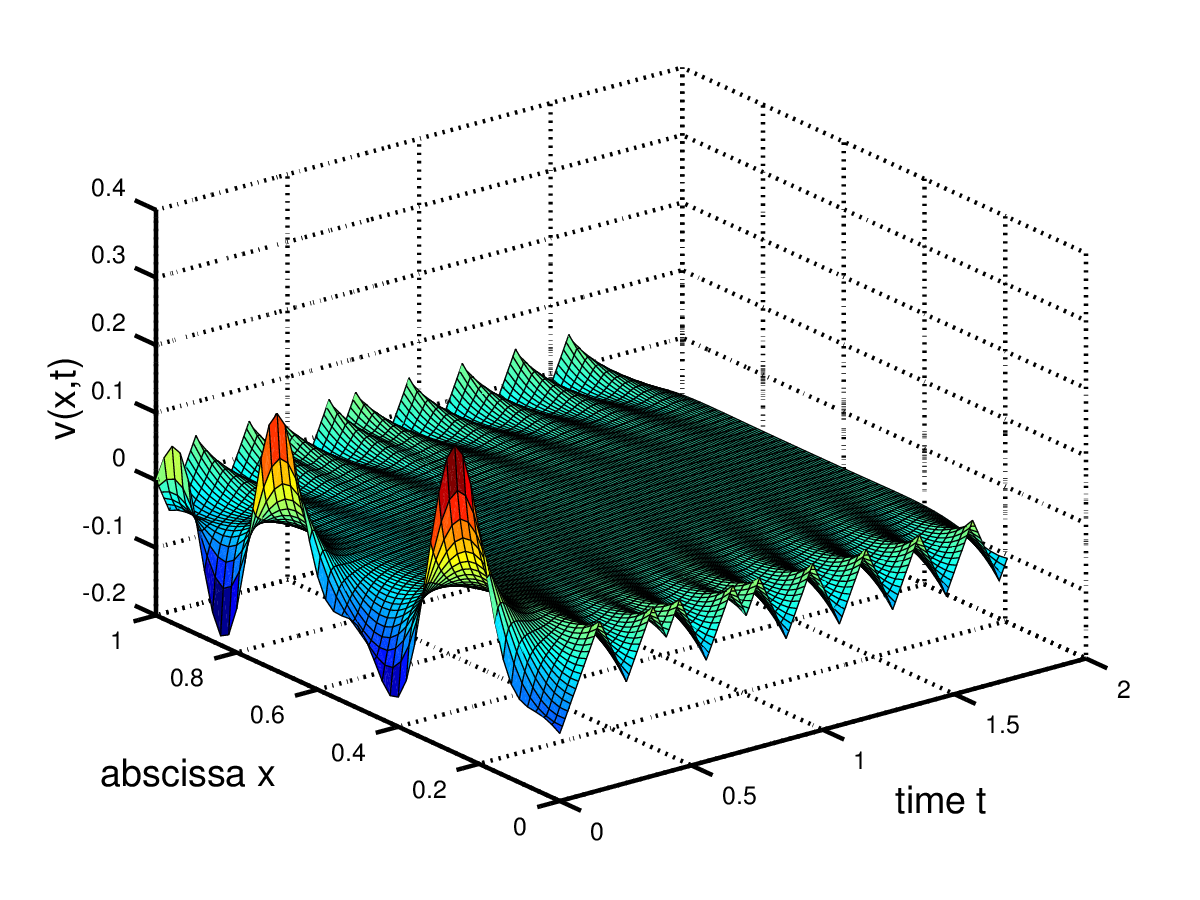
\includegraphics[width=0.8\textwidth]{simu.png}
 \caption{Simulation of the controller.}
 \label{fig:simu_pde}
\end{figure}


%================================================
%
\section{Reliable measurements, online control, and other applications}
%=============================================
%
\section{Discussion}
%==================
%
%\section{Numerical experiments}
%=============================
%
%\section{Extension to the nonlinear case}
%=======================================
%
%
% \begin{thebibliography}{0}
% %
% \end{thebibliography}
% %{\color{red} TOUTES LES VARIABLES A DEFINIR}
% %=========
% %=========
% \end{document}
% 
% 
% 
% 
% 
% 
% 
% 
% 
% 
% 
% 
% 
% 
% 
% 
% 
% 
% 
% 
% 
% 
% 
% 
% 
% 
% 
% 
% 
% 
% 
% 
% 
% 
% 
% 
% 
% 
% 
% 
% 
% 
% 
% 
% 
% 
% 
% 
% 
% 
% 
% 
% 
% 
% 
% 
% 
% 
% 
% 
% 
% 
% 
% 
% 
% 
% 
% 
% 
% 
% 
% 
% 
% 
% 
% 
% 
% 
% 
% 
% 
% 
% 
% 
% 
% 
% 
% 
% 
% 
% 
% 
% 
% 
% 
% 
% 
% 
% 
% 
% 
% 
% 
% 
% 
% 
% 
% 
% 
% 
% 
% 
% 
% %
% \section{Introduction}
% %
% On considère les solutions du problème $(\mathcal{P}_\alpha)$ paramétré par 
% $\alpha\in I\subset\mathbb{R}^+$, $\mathop{mes}(I)<+\infty$~:
% %
% \begin{eqnarray}
% && -\Delta u_\alpha + \alpha\, u_\alpha = f \quad \mbox{ dans } \Omega, \\ [1.1ex]
% && u_\alpha = 0 \quad \mbox{ sur } \partial\Omega.
% \end{eqnarray}
% %
% Cette fois, nous avons un opérateur qui dépend lui-même des paramètres (ici $\alpha$).
% Nous ne pouvons rien décomposer a priori par l'approche EIM. Nous devons construire
% un algorithme qui à la fois cherche un échantillonnage de $\alpha$, calcule des solutions
% du problème $(\mathcal{P}_\alpha)$ et construit une base spatiale réduite. On va construire une suite d'espaces d'approximation de plus en plus grand qui va réduire l'erreur au fur et à 
% mesure de la phase d'enrichissement. \bigskip
% 
% \section{Approche incrémentale gloutonne (greedy)}
% %================================================
% 
% Pour commencer, on se donne $\alpha_1\in I$ quelconque. On note $u_1=u_{\alpha_1}$ solution
% du problème $(\mathcal{P}_{\alpha_1})$. L'espace d'approximation $W^{(1)}$ à l'itération $(1)$,
% est donné par
% \[
% W^{(1)} = \mathop{vect}(\varphi^1), \quad \varphi^1 = \frac{u_1}{\|u_1\|}\in H^1_0(\Omega).
% \]
% La formulation variationnelle de $(\mathcal{P}_\alpha)$ s'écrit
% %
% \begin{equation}
% (\nabla u_\alpha,\nabla v) + \alpha\, (u_\alpha,v) = (f,v)\quad \forall v\in V=H^1_0(\Omega),
% \label{eq:3}
% \end{equation}
% %
% avec $(.,.)$ désignant le produit scalaire dans $L^2(\Omega)$. 
% %
% La formulation variationnelle du problème discret défini sur $W^{(1)}$ s'écrit~: trouver 
% $\tilde u^{(1)}_\alpha$ solution du problème
% %
% \begin{equation}
% (\nabla \tilde u^{(1)}_\alpha,\nabla w) + \alpha\, (\tilde u^{(1)}_\alpha,w) = (f,w)
% \quad \forall w\in W^{(1)}.
% \label{eq:4}
% \end{equation}
% %
% Le problème~\eqref{eq:3} s'écrit de manière équivalente
% \begin{equation}
% (\nabla (u_\alpha-\tilde u_\alpha^{(1)}), \nabla v) + \alpha\, (u_\alpha-\tilde u_\alpha^{(1)},v)
% = (f,v)-(\nabla \tilde u_\alpha^{(1)},\nabla v)-\alpha\,(\tilde u^{(1)}_\alpha,v) \quad \forall v\in V.
% \label{eq:5}
% \end{equation}
% %
% Dans le membre de gauche de~\eqref{eq:5}, on voit apparaître la fonction d'erreur
% \[
% e_\alpha^{(1)}:= u_\alpha - \tilde u_\alpha^{(1)}
% \]
% tandis que dans le membre de droite on voit apparaître un résidu d'équation relatif à 
% la solution approchée $\tilde u^{(1)}$. On définit le résidu à l'itération $(1)$ évalué sur la
% fonction test $v$~:
% \[
% r^{(1)}_\alpha(v) := (f,v)-(\nabla \tilde u_\alpha^{(1)},\nabla v)-\alpha\,(\tilde u^{(1)}_\alpha,v).
% \]
% On remarque que $r^{(1)}$ définit une forme linéaire sur $V$. Sa norme sur l'espace dual $V'$
% est donnée par
% \[
% \|r^{(1)}_\alpha\|_{V'} = \sup_{v\in V, v\neq 0} \ \frac{|r^{(1)}_\alpha(v)|}{\|v\|_V}.
% \]
% On a le résultat suivant~:
% \begin{lemma}
% Pour $\alpha = \alpha_1$, le résidu $r^{(1)}_{\alpha_1}$ est nul et $\tilde u^{(1)}_{\alpha_1}=u_1$. 
% \end{lemma}
% \begin{proof}
% \`A $\alpha=\alpha_1$, $u_1=u_{\alpha_1}$ est la solution du problème
% \[
% (\nabla u_1,\nabla v) + \alpha_1\, (u_1,v) = (f,v)\quad \forall v\in V.
% \]
% La solution approchée $\tilde u^{(1)}_{\alpha_1}\in W^{(1)}$ est solution de 
% %
% \begin{equation}
% (\nabla \tilde u^{(1)}_{\alpha_1},\nabla w) + \alpha_1\, (\tilde u^{(1)}_{\alpha_1},w) = (f,w)
% \quad \forall w\in W^{(1)}=\mathop{vect}(u_1).
% \label{eq:4}
% \end{equation}
% La fonction $w=u_1-\tilde u^{(1)}_{\alpha_1}$ reste dans $W^{(1)}$, si bien que l'on a
% \[
% \|\nabla (u_1-\tilde u^{(1)}_{\alpha_1})\|^2 + \alpha_1 \, 
% \|u_1-\tilde u^{(1)}_{\alpha_1}\|^2 = 0
% \]
% d'où $u_1=\tilde u^{(1)}_{\alpha_1}$ et $r^{(1)}_{\alpha_1}(v) = 0$ pour tout $v\in V$.
% \end{proof}
% %
% Il convient alors de déterminer le nouveau point $\alpha=\alpha_2$ qui maximise le résidu
% (pire cas) pour enrichir la base discrète:
% \[
% \alpha_2 = \arg \max_{\alpha\in I}\quad  \| r_\alpha^{(1)}\|_{V'}
% \]
% On calcule alors $u_2$ solution de
% %
% \begin{equation}
% (\nabla u_2,\nabla v) + \alpha_2\, (u_2,v) = (f,v)\quad \forall v\in V,
% \label{eq:3}
% \end{equation}
% %
% puis on prend 
% \[
% \varphi^{(2)} = \frac{u_2}{\|u_2\|}, 
% \]
% et
% \[
% W^{(2)} = \mathop{vect}(\varphi^1,\, \varphi^2),
% \]
% %
% le nouveau modèle réduit s'écrivant 
% %
% \begin{equation}
% (\nabla \tilde u^{(2)}_\alpha,\nabla w) + \alpha\, (\tilde u^{(2)}_\alpha,w) = (f,w)
% \quad \forall w\in W^{(2)}.
% \label{eq:8}
% \end{equation}
% %
% etc ... On s'arrête au rang $M$ quand on atteint le critère
% \[
% \max_{\alpha\in I}\quad \|r_\alpha^{(M)}\| < \varepsilon_{tol}.
% \]
% On obtient au rang $(M)$ une base réduite de rang $M$ et un espace d'approximation
% \[
% W^{(M)} = \mathop{vect}\left( \varphi^1, ..., \varphi^M \right).
% \]
% La solution réduite sera recherchée de la forme
% \[
% \tilde u^{(M)}_\alpha(x) = \sum_{m=1}^M \ \beta_m(\alpha)\, \varphi^m(x)
% \]
% et solution de 
% \begin{equation}
% (\nabla \tilde u^{(M)}_\alpha,\nabla w) + \alpha\, (\tilde u^{(M)}_\alpha,w) = (f,w)
% \quad \forall w\in W^{(M)}.
% \label{eq:9}
% \end{equation}
% %
% En notant $\bm{\beta}(\alpha)=(\beta_m(\alpha))_m\in\mathbb{R}^m$, le problème d'ordre réduit
% s'écrira
% \[
% \left(A + \alpha\, M\right)\bm{\beta}(\alpha) = \bm{F}
% \]
% avec $A,M\in\mathscr{M}_M(\mathbb{R})$ symétriques définies positives. Si on peut procéder
% à l'inversion symbolique de la matrice $(A+\alpha M)$ par rapport à la variable $\alpha$,
% on obtient alors les coefficients de manière symbolique
% \[
% \bm{\beta}(\alpha) = (A+\alpha M)^{-1} \bm{F}.
% \]
% La solution réduite est alors
% \[
% \tilde u^{(M)}_\alpha(x) = \sum_{m=1}^M \ \left((A+\alpha M)^{-1} \bm{F}\right)_m\ \varphi^m(x).
% \]
% %
% \section{Réduction de modèle de deuxième niveau (stage 2)}
% %=========================================================
% %
% Maintenant que l'on possède une solution réduite explicite $\tilde u^{(M)}_\alpha$,
% on peut s'intéresser à un procédé d'interpolation empirique (EIM) pour construire
% une base dans l'espace paramétrique. \bigskip
% 
% On cherche d'abord
% \[
% x_1 = \arg \max_{x\in\bar\Omega}\quad \|\tilde u^{(M)}_\alpha(x)\|_{L^\infty(I)}
% \] 
% puis 
% \[
% \hat \alpha_1 = \arg\max_{\alpha\in I}\quad  |\tilde u^{(M)}_\alpha(x_1)|.
% \]
% Si besoin, on ajoute au plan d'expérience la solution exacte $\hat u_1 = u_{\hat \alpha_1}$
% (offline). On obtient alors le premier mode paramétrique
% \[
% q_1(\alpha) = \frac{\tilde u_\alpha^{(M)}(x_1;\alpha)}{\tilde u_\alpha^{(M)}(x_1;\hat \alpha_1)}
% \]
% et un premier opérateur d'interpolation en la variable $\alpha$~:
% \[
% \mathscr{I}^{(1)}u(\alpha) = u(\hat \alpha_1)\, q_1(\alpha).
% \]
% De proche en proche, on obtient une famille de points d'interpolation
% $(\hat \alpha_1,\hat\alpha_2,...,\hat\alpha_K)$ et de modes paramétriques
% $(q_1(\alpha),q_2(\alpha),...,q_K(\alpha))$ que l'on peut arranger pour satisfaire
% la propriété de Lagrange, i.e.
% \[
% q_k(\hat\alpha_\ell) = \delta_{k\ell}.
% \] 
% On obtient alors le modèle réduit de deuxième niveau, totalement explicite
% \[
% \hat u_\alpha(x) = \sum_{k=1}^K \hat u_k(x)\, q_k(\alpha).
% \]
% On pourra remarquer que ce modèle réduit est interpolant, et vaut la solution exacte
% $\hat u_k(x)$ pour chaque paramètre $\alpha=\hat\alpha_k$.
% %
% \end{document}
% 
% 
% 
% 
% 
% 
% 
% 
% 
% 
% 
% 
% 
% 
% 
% 
% 
% 
% 
% 
% 
% 
% 
% 
% 
% 
% 
% 
% 
% 
% 
% 
% 
% 
% 
% 
% 
% 
% 
% 
% 
% 
% 
% 
% 
% 
% 
% 
% 
% 
% 
% 
% 
% 
% 
% 
% 
% 
% 
% 
% 
% {\bf Notations:} 
% 
% Vectors are in bold, scalars are not.
% 
% We denote by $\Omega = [0,1]$ the domain of definition of the PDE.
% 
% We denote by $\partial \Omega$ the boundary of $\Omega$.
% 
% We denote by $L^2(\Omega)$ the space of square integrable functions on $\Omega$.
% 
% The associated scalar product on $\Omega$ is defined by $( f,g )_\Omega = \int_\Omega f(x) g(x) dx$.
% 
% We denote by $\Vert \cdot \Vert_\Omega$ the associated norm (sometimes called $L^2$ norm), 
% {\em i.e.:} $\Vert f \Vert_\Omega = \sqrt{(f,f)_\Omega}$.
% 
% We define the Sobolev space $H^1 (\Omega) = \{ v \in L^2(\Omega),\ \dfrac{\partial v}{\partial x} \in L^2(\Omega) \}$
% 
% We define the Sobolev space $H^1_0 (\Omega) = \{ v \in H^1(\Omega), \ v_{| \partial \Omega} = 0   \}$
% 
% 
% 
% 
% 
% 
% 
% 
% 
% 
% 
% \section{Problem statement}
% 
% We wish to consider the equation system (\ref{eq:ODE}-\ref{eq:PDE}-\ref{eq:BC1}-\ref{eq:BC2}-\ref{eq:IC}) 
% given by:
% \begin{itemize}
%  \item an ODE of dimension 2 ($\bx \in \mathbb{R}^2$):
% \begin{eqnarray}
%  && \dot{\bm{a}} = \bm{b}_u
%  \label{eq:ODE}
% \end{eqnarray}
% 
% \item a parabolic PDE:
% \begin{equation}
%  \alpha \dfrac{\partial v}{ \partial t} -  \dfrac{\partial^2 v}{ \partial x^2} = 0 \quad\mbox{ in } \Omega 
% \label{eq:PDE}
%  \end{equation}
% with Dirichlet boundary conditions 
% \begin{eqnarray}
% && v(0,t) = a_1(t) \label{eq:BC1} \\
% && v(1,t) = a_2(t)
% \label{eq:BC2}
% \end{eqnarray}
% and an initial condition
% \begin{equation}
%  v(\cdot,0) = v_0.
%  \label{eq:IC}
% \end{equation}
% 
% 
% \end{itemize}
% 
% The state of the system is given by $(\ba,v)$.
% The ODE is controlled by a control input $u$ belonging to a finite set $U = \{1,2,3,4\}$.
% System (\ref{eq:ODE}-\ref{eq:PDE}-\ref{eq:BC1}-\ref{eq:BC2}-\ref{eq:IC}) is thus a switched controlled system.
% We suppose that switchings occur periodically, every $\tau$ seconds.
% 
% We suppose that we have four switched modes: 
% 
% $\bm{b}_1 = \left( \begin{array}{c}1\\1\end{array} \right)$ , $\bm{b}_2 = \left( \begin{array}{c}-1\\-1\end{array} \right)$,
% $\bm{b}_3 = \left( \begin{array}{c}-1\\1\end{array} \right)$, $\bm{b}_4=\left( \begin{array}{c}1\\-1\end{array} \right)$
% 
% Given an objective state $\bar v$, the objective is to compute
% a control rule $\tilde u(t)$ so that the state $v(x,t)$ of the PDE
% stays (or goes) as close as possible to $\bar v$ in $L^2(\Omega)$ norm.
% % , {\em i.e.}, for some $\varepsilon >0$:
% % \begin{equation}
% %  \forall t \geq 0, \quad \Vert v(\cdot,t) - \bar v \Vert_\Omega \leq \varepsilon
% % \end{equation}
% % or
% % \begin{equation}
% %  \exists t>0, \forall t'\geq t,\quad  \Vert v(\cdot,t') - \bar v \Vert_\Omega \leq \varepsilon
% % \end{equation}
% 
% We would like 
% to synthesize a state-dependent switching rule, i.e. $\tilde u(t) = \tilde u((\ba(t),v(t)))$.
% The control problem is formalized as follows:
% 
% \begin{problem}[Stability]
%  Let us consider the equation system (\ref{eq:ODE}-\ref{eq:PDE}-\ref{eq:BC1}-\ref{eq:BC2}-\ref{eq:IC}).
%  Given a tolerance $\varepsilon$, synthesize a state-dependent switching rule $\tilde u((\ba(t),v(t)))$
%  such that, for all initial condition $v_0$ verifying $\Vert v_0 - \bar v \Vert_\Omega \leq \varepsilon$, we have:
%  \begin{equation}
%  \forall t \geq 0, \quad \Vert v(\cdot,t) - \bar v \Vert_\Omega \leq \varepsilon
% \end{equation}
%  \label{prob:control} 
% \end{problem}
% 
% 
% \begin{problem}[Reachability]
%  Let us consider the equation system (\ref{eq:ODE}-\ref{eq:PDE}-\ref{eq:BC1}-\ref{eq:BC2}-\ref{eq:IC}).
%  Given tolerances $\varepsilon_1$ and $\varepsilon_2$ with $\varepsilon_1 > \varepsilon_2$, 
%  synthesize a state-dependent switching rule $\tilde u((\ba(t),v(t)))$
%  such that, for all initial condition $v_0$ verifying $\Vert v_0 - \bar v \Vert_\Omega \leq \varepsilon_1$, 
%  we have 
% \begin{equation}
%  \exists t>0, \forall t'\geq t,\quad  \Vert v(\cdot,t') - \bar v \Vert_\Omega \leq \varepsilon_2
% \end{equation}
%  \label{prob:control2} 
% \end{problem}
% 
% 
% 
% 
% 
% \section{Symbolic control (old)}
% Control synthesis by state-space decomposition (MINIMATOR).
% Available for systems of the form (\ref{eq:symbolic}).
% 
% 
% Permits to send a set of states $R$ (a box of $\mathbb{R}^m$) to
% a target set $R_{t}$ (a box of $\mathbb{R}^m$).
% 
% The state of a PDE is of infinite dimension. Supposing that a finite element discretization is used, 
% the state dimension is finite, but much higher than what can be handled by guaranteed symbolic 
% methods. We thus need thus need  a Model Order Reduction in order to reduce the state
% dimension.
% 
% 
% \section{Spectral Model Reduction}
% \label{sec:ROM}
% 
% We wish to approximate the state $v(x,t)$ of the PDE by a 
% state $\tilde v (x,t)$ as close as possible to $v(x,t)$, 
% but which can be computed much more easily than by solving the PDE (e.g. with a finite element
% method). A natural way of computing an approximate solution 
% of (\ref{eq:PDE}) is using a modal (spectral) decomposition [ref?].
% An accurate approximate solution of (\ref{eq:PDE}) can be obtained with few 
% eigen modes when the boundary conditions are homogeneous. 
% We thus introduce the lifting $v_l(x,t)=a_1(t)(1-x) + a_2(t)x$.
% Writing 
% $$
%   v(x,t) = v_l(x,t) + w(x,t)
% $$
% and injecting it in (\ref{eq:PDE}-\ref{eq:BC1}-\ref{eq:BC2}-\ref{eq:IC}) gives
% \begin{equation}
%  \alpha \dfrac{\partial w}{ \partial t} -  \dfrac{\partial^2 w}{ \partial x^2} = -\alpha \dfrac{\partial v_l }{\partial t} \quad\mbox{ in } \Omega 
% \label{eq:PDE2}
%  \end{equation}
% with Dirichlet boundary conditions 
% \begin{eqnarray}
% && w(0,t) = 0 \label{eq:BC12} \\
% && w(1,t) = 0
% \label{eq:BC22}
% \end{eqnarray}
% and an initial condition
% \begin{equation}
%  w(\cdot,0) = v_0 - v_l(\cdot,0).
%  \label{eq:IC2}
% \end{equation}
% 
% 
% 
% We can thus look for a reduced model of the form
% \begin{equation}
%  \tilde v(x,t) = v_l(x,t) + \tilde w(x,t)
%  \label{eq:vtilde}
% \end{equation}
% 
% If we furthermore look for solutions for $w$ (or $\tilde w$) with separated variables 
% (of the form $\beta(t) \phi(x)$), we obtain an eigenvalue problem $\phi'' = \mu \phi$,
% which has an infinite number of solutions $\{ \varphi_i \}_{i = 1,\dots,+\infty }$.
% %
% % \begin{equation}
% % \tilde v(x,t) =  a_1(t)(1-x) + a_2(t)x + \sum_{i = 1}^N \beta_i (t) \varphi_i (x)
% % \label{eq:ROM}
% % \end{equation}
% % 
% % where the $\beta_i$ are the time coefficients associated to the space functions $\varphi_i$,
% % which are precomputed (the computation of the $\varphi_i$ is detailed in
% % the following). 
% % 
% % Let us explain why the lifting is interesting. 
% % If we write $\tilde v(x,t) =  a_1(t)(1-x) + a_2(t)x + w(x,t)$ and inject it in (\ref{eq:PDE},\ref{eq:BC1},\ref{eq:BC2}),
% % we have:
% % 
% % 
% % \begin{align*}
% % & \alpha \dfrac{\partial \tilde v}{ \partial t} -  \dfrac{\partial^2 \tilde v}{ \partial x^2} = 0 \quad\mbox{ in } \Omega \\
% % & \tilde v (0,t) = a_1(t) \\
% % & \tilde v (1,t) = a_2(t)
% % \end{align*}
% % 
% % 
% % \begin{align*} 
% % & \alpha \left( \dot a_1(t)(1-x) + \dot a_2(t)x + \dfrac{\partial w}{ \partial t} \right) -  \dfrac{\partial^2 w}{ \partial x^2} = 0 \quad\mbox{ in } \Omega \\
% % & w(0,t) + a_1(t) = a_1(t) \\
% % & w (1,t) + a_2(t) = a_2(t)
% % \end{align*}
% % 
% % \begin{align*}
% % & \alpha \dfrac{\partial w}{ \partial t}  -  \dfrac{\partial^2 w}{ \partial x^2} = -\alpha ( \dot a_1(t)(1-x) + \dot a_2(t)x) \quad\mbox{ in } \Omega \\
% % & w(0,t) = 0 \\
% % & w(1,t) = 0
% % \end{align*}
% % 
% % 
% % The lifting $a_1(t)(1-x) + a_2(t)x$ permits to obtain homogeneous boundary conditions
% % for $w$.
% The eigenvalue problem $\phi'' = \mu \phi$ with homogeneous boundary 
% conditions leads to eigenmodes (see \cite{cain2005separation}):
% \begin{equation}
% \varphi_i(x) = \sqrt{2} \sin{(i \pi x)}
% \label{eq:modes}
% \end{equation}
% Note that the eigenmodes $\varphi_i$ have been normalized w.r.t.
% the scalar product $(\cdot , \cdot )_\Omega$.
% It can be shown that a solution for $w$ can be decomposed on the basis of 
% the eigenmodes $w(x,t) = \sum_{i=1}^\infty \beta_i(t)\varphi_i(x)$.
% % Having written $w$ under this last form,
% % an exact solution for equations (\ref{eq:PDE},\ref{eq:BC1},\ref{eq:BC2}) can be found as
% % \begin{equation}
% % \alpha \dfrac{\partial w}{ \partial t}  -  \dfrac{\partial^2 w}{ \partial x^2} = -\alpha \sum_{i=0}^\infty (  \dfrac{\partial v_l}{\partial t}   , \varphi_i )_\Omega \varphi_i
% % \end{equation}
% % % 
% 
% \begin{theorem}
%  Let $w$ be a solution of (\ref{eq:PDE2},\ref{eq:BC12},\ref{eq:BC22}) with initial condition $w_0$. We have:
%  \begin{equation}
%   w(x,t) = \sum_{i=1}^\infty \beta_i(t)\varphi_i(x)
%   \label{eq:exact_sol}
%  \end{equation}
%   
%  with, for all $i \geq 0$:
%  $$
%  \varphi_i(x) = \sqrt{2} \sin{(i \pi x)}
%  $$
%  and 
%  $$ 
%   \beta_i (t) = e^{-(i\pi)^2t} (w_0,\varphi_i)_\Omega - \int_0^t e^{-(i\pi)^2(t-s)} (\dot v_l(\cdot,s),\varphi_i)_\Omega ds
%  $$
% \end{theorem}
% \begin{proof}
%  See [ref]
% \end{proof}
% 
% 
% 
% % Using a modal decomposition means that 
% % the functions $\varphi_i$ are computed as the eigenmodes of this last equation system
% % (\ref{eq:PDE_homo1} - \ref{eq:PDE_homo3}), see \cite{cain2005separation} for details of the computation (NB: we normalize it w.r.t. 
% % the scalar product $\langle \cdot , \cdot \rangle_\Omega$).
% % To obtain an exact solution, we should make $N$ tend to infinity, but one can 
% % often use only few functions to accurately represent the solution. 
% % We have: 
% 
% 
% Instead of searching an exact solution, 
% we will look for an approximate solution by truncating the sum \eqref{eq:exact_sol} at
% an order~$N$, that is
% \begin{equation}
%  \tilde w(x,t) = \sum_{i=1}^N \beta_i(t)\varphi_i(x)
%  \label{eq:wtilde}
% \end{equation}
%  with, for all $i = 1, \dots, N$:
%  $$
%  \varphi_i(x) = \sqrt{2} \sin{(i \pi x)}
%  $$
%  and 
%  $$ 
%  \beta_i (t) = e^{-(i\pi)^2t} (w_0,\varphi_i)_\Omega - \int_0^t e^{-(i\pi)^2(t-s)} (\dot v_l(\cdot,s),\varphi_i)_\Omega ds
%  $$
% 
% In fact, $\tilde w$ is a projection of $w$ on $span\{\varphi_1,\dots, \varphi_N\}$. We will
% denote the associated projector by $P_N$. 
% % 
% % Let us now explain how we can compute an approximate solution
% % $\tilde v(x,t)$ of the form (\ref{eq:vtilde}), solution 
% % of the equation system (\ref{eq:PDE2},\ref{eq:BC12},\ref{eq:BC22}).
% % We have:
% % 
% % $$ \alpha \dfrac{\partial \tilde v}{ \partial t} -  \dfrac{\partial^2 \tilde v}{ \partial x^2} = 0 \quad\mbox{ in } \Omega $$
% % 
% % $$ \alpha \dfrac{\partial \tilde v}{ \partial t} w -  \dfrac{\partial^2 \tilde v}{ \partial x^2}w = 0  \quad\mbox{ in } \Omega \quad \forall w \in H^1_0(\Omega)$$
% % 
% % Writing the weak form formulation and using an integration by parts, we obtain:
% % 
% % $$ \alpha \dfrac{d}{dt} ( \tilde v,w)_\Omega + (\dfrac{\partial \tilde v}{\partial x}, \dfrac{\partial w}{\partial x})_\Omega = 0 \quad \forall w \in H_0^1(\Omega) $$
% % 
% % This is true for all $w \in H_0^1(\Omega)$, we can thus write:
% % 
% % $$\displaystyle{ \alpha \dfrac{d}{dt} (\tilde v, w)_\Omega + (\dfrac{\partial \tilde v}{\partial x}, \dfrac{\partial w}{\partial x})_\Omega =0, \quad \forall w \in W^k = \text{Vect}(\varphi_k)}$$
% % 
% % Which leads to:
% % 
% %  \begin{multline*}
% %  \displaystyle{ \alpha \int_\Omega ((1-x) \dot a_1 + x \dot a_2) \varphi_k dx + \int_\Omega ((1-x) a_1 + x a_2) \dfrac{\partial \varphi_k}{\partial x} dx } \\ 
% %  \displaystyle{+ \alpha \sum_{i=1}^N \dot \beta_i \int_\Omega \varphi_i \varphi_k dx + \sum_{i=1}^N \beta_i \int_\Omega \dfrac{ \partial \varphi_i}{\partial x} \dfrac{ \partial \varphi_k}{\partial x} dx = 0, \quad \forall k = 1,\dots,N}
% %  \end{multline*}
% % 
% % \vspace{1em}
% % 
% % The second term being equal to zero, we then have a low dimensional equation:
% % \begin{equation}
% %  \alpha C_r \dot{\bm{\beta}} + K_r \bm{\beta} = - \alpha \bm{F_r}(\dot{\bm{a}},t)
% %  \label{eq:red}
% % \end{equation}
% % 
% % with $\bm{\beta}$ the vector composed of the $\beta_i$, which we call 
% % the reduced state, $C_{r,ij} = \int_\Omega  \varphi_i \varphi_j dx$, $K_{r,ij} = \int_\Omega  \dfrac{ \partial \varphi_i}{\partial x} \dfrac{ \partial \varphi_j}{\partial x} dx$
% % and ${F_{r,i}}(\dot{\bm{a}},t) = \int_\Omega ((1-x) \dot a_1 + x \dot a_2) \varphi_i dx$.
% % Note here that matrices $C_r$ and $K_r$ are diagonal, because functions $\varphi_i$
% % are orthogonal. This is one of the main advantages
% % in using such a modal decomposition: an accurate approximate solution
% % can be computed in a very cheap way.
% % 
% % Solving the equation system (\ref{eq:ODE}-\ref{eq:PDE}-\ref{eq:BC1}-\ref{eq:BC2})
% % with the reduced order solution (\ref{eq:ROM}) then leads to solving
% % the reduced system:
% % 
% % 
% % \begin{equation}
% % \label{eq:sys_red}
% %   \left( \begin{array}{c}
% %   \dot{\bm{a}}(t) \\ \dot{\bm{\beta}}(t)
% %  \end{array} \right) = \left( \begin{matrix} 0 & 0 \\ 0 & 1/\alpha C_r^{-1} K_r \end{matrix} \right)\left( \begin{array}{c}
% %    \bm{a}(t) \\ \bm{\beta}(t)
% %  \end{array} \right) + \begin{pmatrix}
% %                         \bm{b}_u(t) \\ -C_r^{-1} \bm{F_r}(\bm{b}_u(t),t)
% %                        \end{pmatrix}
% % \end{equation}
% % 
% % 
% % 
% % However, although the lifting $a_1(t)(1-x) + a_2(t)x$ permits to construct an accurate reduced model 
% % with few functions $\varphi_i$, it raises a new problem:
% % the coefficients $\beta_i$ have no physical meaning. 
% % It is thus not trivial to infer a reduced objective (a box, or an objective set)
% % for the reduced state $\bm{\beta}$. In other words, we do not know 
% % where the $\beta_i$ should stabilize to obtain a PDE state as close to zero as we want. 
% 
% 
% \section{Error bounding}
% \label{sec:bound}
% 
% 
%  
%  \begin{proposition}
%   Let $E(t) = \int_0^L | v(x,t) - \tilde v(x,t) |^2 dx$
%  with $v$ solution of (\ref{eq:PDE}-\ref{eq:BC2}) with an initial condition
%  $v_0 \in L^2 (\Omega)$ and a fixed $\ba(\cdot)$ trajectory, 
%  and $\tilde v$ the associated approximate solution of the form (\ref{eq:ROM}).
%  We denote by $P_N$ the projection on $\text{span}\{ \varphi_i,\ 1\leq i \leq N \}$.
% We have, for all $t \in [0,k\tau]$:
% \begin{multline}
%  E(t) \leq \| v_0 - P_N v_0 \|^2 e^{-(\pi )^2t} 
%  +
% \left( \dfrac{1}{\pi} \right) ^2  \int_0^t e^{-(\pi / 1)^2 (t-s)} \left \lbrack \| G(x,s) - P_N G(x,s) \|^2  \right \rbrack ds
% \end{multline}
% with $G(x,t) = - \alpha (\dot{a_1}(t) (1-x) + \dot{a_2} (t) x)$ in $\Omega \times [0,k\tau]$.
%  \end{proposition}
% 
% \begin{proof}
% Let $\bm{b}_{u_1},\dots,\bm{b}_{u_K}$ be a fixed switching sequence and
% $\ba (0)\in \mathbb{R}^2$ so that we have a fixed trajectory 
% $\ba (t)$ for $t \in [0,K\tau]$.
% 
% Let $v$ be solution of (\ref{eq:PDE},\ref{eq:BC1},\ref{eq:BC2}) 
% with an initial condition $v(x,0) = v_0(x) \in L^2(\Omega)$ and the fixed $\ba(\cdot)$
% trajectory.
% 
% Let $k(x,t) = (1-x)a_1(t) + xa_2(t)$.
% 
% Let $\tilde v(x,t) = v_N(x,t) = (1-x)a_1(t) + xa_2(t) + \sum_{i=1}^N \beta_i(t) \varphi_i(x)$ be
% the approximate solution. 
% % with $\bm{\beta}$ computed with (\ref{eq:red}).
% 
% We can write
% $$ v(x,t) = w(x,t) + v_l(x,t) $$
% and
% $$ v_N(x,t) = w_N(x,t) + v_l(x,t). $$
% 
% % Then $w_N(x,t) = \sum_{i=1}^N \beta_i(t) \varphi_i(x)  = P_N w(x,t)$.
% 
% The convergence of $v_N$ to $v$ when $N \longrightarrow \infty$ is equivalent to the convergence of $w_N$ to $w$.
% With lifting $k$ written as above, $w$ verifies the equation system:
% 
% \begin{align*}
% & \alpha \dfrac{\partial w}{ \partial t}  -  \dfrac{\partial^2 w}{ \partial x^2} = -\alpha ( \dot a_1(t)(1-x) + \dot a_2(t)x) ) G(x,t) \quad\mbox{ in } \Omega \\
% & w(0,t) = 0 \\
% & w(1,t) = 0 \\
% & w(x,0) = v_0(x)- v_l(x,0) := w_0(x)
% \end{align*}
% 
% and $w_N$ is solution of the equation system:
% \begin{align*}
% & \alpha \dfrac{\partial w_N}{ \partial t}  -  \dfrac{\partial^2 w_N}{ \partial x^2} = P_NG(x,t) \quad\mbox{ in } \Omega \\
% & w_N(0,t) = 0 \\
% & w_N(1,t) = 0 \\
% & w_N(x,0) = (P_N w_0)(x)
% \end{align*}
% 
% Note that the first line is equivalent to the equation (\ref{eq:red}) (equation (\ref{eq:red})
% is an identification of the basis coefficients associated to the basis $(\varphi_i)_{i=1,\dots,N}$ of the
% first line above).
% Let 
% $$
% e(x,t) = w(x,t) - w_N(x,t)
% $$
% denote the error of the approximation. Then $e(x,t)$ is the solution of 
% $$
% \dfrac{\partial^2 e}{\partial x^2} - \dfrac{\partial e }{\partial t} = G(x,t) - P_NG(x,t) 
% $$
% $$
% e(0,t) = e(L,t) = 0
% $$
% $$
% e(x,0) = w_0(x) - P_N w_0(x)
% $$
% 
% If we multiply the differential equation by $e(x,t)$ and integrate w.r.t. $x$, we obtain
% $$
% \int_\Omega \left( \dfrac{\partial^2 e}{\partial x^2} - \dfrac{\partial e }{\partial t} \right)e\ dx = \int_\Omega [G - P_NG]e\ dx
% $$
% After integrating the first term by parts the following equation results:
% $$
% \dfrac{1}{2} \dfrac{d}{dt} \int_\Omega e^2(x,t)dx = - \int_\Omega \left( \dfrac{\partial e}{\partial x} \right)^2 - \int_\Omega [G - P_N G] e(x,t) dx.
% $$
% Besides, we have:
% $$
% \int_\Omega e(x,t)^2 dx \leq \left( \dfrac{1}{\pi} \right) ^2 \int_\Omega \left( \dfrac{\partial e}{\partial x} \right) ^2 dx
% $$
% 
% The inequality allows the following estimate for the mean square error at time $t$:
% \begin{equation}
%  \dfrac{d}{dt} E(t) \leq -2 \pi^2 E(t) + 2 \int_\Omega | G(x,t) - P_N G(x,t) | | e(x,t)| dx
%  \label{eq:error_estimate}
% \end{equation}
% 
% Applying the algebraic-geometric mean inequality 
% $$
% 2 \left( \dfrac{a}{\sqrt{\varepsilon}} \sqrt{\varepsilon} b \right) \leq \dfrac{a^2}{\varepsilon} + \varepsilon b^2
% $$
% with $\varepsilon = \pi^2$ we obtain the estimate 
% $$
% \int_\Omega [G(x,t) - P_N G (x,t)] e(x,t) dx \leq \left( \dfrac{1}{\pi} \right) ^2 \int_\Omega [G(x,t) - P_N G(x,t)]^2 dx + \pi^2 E(t)
% $$
% With the estimate (\ref{eq:error_estimate}) we have the following error bound:
% \begin{equation}
% E'(t) \leq - \pi^2 E(t) + \left( \dfrac{1}{\pi} \right) ^2 \| G - P_N G \|_\Omega ^2
%  \label{eq:bound}
% \end{equation}
% $$
% E(0) = \| w_0 - P_N w_0 \|_\Omega^2
% $$
% where $\| \cdot \|$ is the norm associated to the scalar product $\langle \cdot, \cdot \rangle_\Omega$.
% inequalities like (\ref{eq:bound}) occur frequently in the qualitative study of
% ordinary differential equations. If we express it as 
% an equality:
% $$
% E'(t) =  - \pi^2 E(t) + \left( \dfrac{1}{\pi} \right) ^2 \| G - P_N G \|_\Omega ^2 - g(t)
% $$
% for some nonnegative (but unknown) function $g(t)$, then this equation
% has the solution 
% \begin{multline*}
%  E(t) = \| v_0 - P_N v_0 \|_\Omega^2 e^{-(\pi )^2t} 
%  +
%   \int_0^t e^{-(\pi )^2 (t-s)} \left \lbrack \left( \dfrac{1}{\pi} \right) ^2 \| G(x,s) - P_N G(x,s) \|_\Omega^2 - g(s)  \right \rbrack ds
% \end{multline*}
% Which proves the result.
% \end{proof}
% 
% 
% \begin{proposition}
%  For the selected case study, if we have:
%  \begin{equation}
%   \frac{1}{\pi^4} \Vert \dot v_l - P_N \dot v_l \Vert_\Omega \leq \Vert v_0 - P_N v_0 \Vert_\Omega^2
%  \end{equation}
% 
%  Then we have $E(t) \leq E(0)$ for all $t\leq \tau$.
%   \label{prop:e_t}
% \end{proposition}
% 
% \begin{proof}
%  $$  E(t) \leq E(0) $$
%  is equivalent to
% 
%  $$ \Vert v_0 - P_N v_0 \Vert_\Omega e^{-\pi^2 t} + \int_0^t \frac{1}{\pi^2} e^{\pi^2 (t-s)} \Vert \dot v_l(\cdot,s) - P_N \dot v_l(\cdot,s) \Vert_ \Omega ^2 ds \leq \Vert v_0 - P_N v_0 \Vert_\Omega^2$$
%  
%  In our case, $\dot v_l (\cdot,s)$ is constant by mode.
%  It is thus equivalent to:
%  $$ \Vert v_0 - P_N v_0 \Vert_\Omega e^{-\pi^2 t} + \frac{1 - e^{-\pi^2 t}}{\pi^2}\frac{1}{\pi^2} \Vert \dot v_l(\cdot,s) - P_N \dot v_l(\cdot,s) \Vert_ \Omega ^2 \leq \Vert v_0 - P_N v_0 \Vert_\Omega^2  $$
%  and
%  $$ \frac{1 - e^{-\pi^2 t}}{\pi^2}\frac{1}{\pi^2} \Vert \dot v_l(\cdot,s) - P_N \dot v_l(\cdot,s) \Vert_ \Omega ^2 \leq \Vert v_0 - P_N v_0 \Vert_\Omega^2 ( 1 - e^{-\pi^2 t}) $$
%  \end{proof}
% 
% 
% \section{Application to symbolic control}
% 
% 
% Let $\bar a_1 = \bar v(0)$ and $\bar a_2 = \bar v(1)$
% $$\bar v_l = \bar a_1 (1-x) + \bar a_2 x$$
% and 
% $$\bar w = \bar v - \bar v_l$$
% We have:
% $$ \Vert v(t) - \bar v \Vert_\Omega^2 \leq \Vert v(t) - \tilde v(t) \Vert_\Omega^2 + \Vert \tilde v(t) - \bar v \Vert_\Omega ^2 $$
% 
% $$ \Vert v(t) - \bar v \Vert_\Omega^2 \leq \Vert v(t) - \tilde v(t) \Vert_\Omega^2 + \Vert \tilde w(t) + v_l(t) - \bar w - \bar v_l \Vert_\Omega ^2 $$
% 
% \begin{equation}
%  \Vert v(t) - \bar v \Vert_\Omega^2 \leq \Vert v(t) - \tilde v(t) \Vert_\Omega^2 + \Vert \tilde w(t) - P_N \bar w \Vert_\Omega^2 + \Vert P_N \bar w - \bar w \Vert_\Omega ^2 + \Vert v_l(t) - \bar v_l \Vert_\Omega^2 
%  \label{eq:bound_final}
% \end{equation}
% 
% 
% For a given truncation order, the term $\Vert P_N \bar w - \bar w \Vert_\Omega ^2 = \gamma$ is constant.
% It highlights the fact that the (non lifting part of the) objective $\bar w$ cannot be represented as 
% precisely as one can want with a given truncation order.
% Under the conditions of Proposition \ref{prop:e_t}, the term 
% $\Vert v(t) - \tilde v(t) \Vert_\Omega^2 = E(t) \leq E(0)$ is 
% a tolerance on the accuracy with which one can represent an initial 
% condition.
% The terms $\Vert \tilde w(t) - P_N \bar w \Vert_\Omega^2$ and $\Vert v_l - \bar v_l \Vert_\Omega^2$ are the terms we control. 
% Let us write
% $P_N \bar w(x) = \sum_{k=1}^N \bar \beta_k \varphi_k (x)$. We have:
% $$ \Vert \tilde w(t) - P_N \bar w \Vert_\Omega^2 = \Vert  \sum_{k=1}^N \beta_k(t) \varphi_k (x) - \sum_{k=1}^N \bar \beta_k \varphi_k (x)\Vert_\Omega^2 $$
% The eigen modes $\varphi_k$ being orthonormal, we get:
% $$ \Vert \tilde w(t) - P_N \bar w \Vert_\Omega^2 =   \sum_{k=1}^N \Vert \beta_k(t)-  \bar \beta_k \Vert^2 $$
% which is an Euclidean norm. 
% 
% Besides, in our case:
% 
% $$ \displaystyle{ \| v_l(t) - \bar v_l \|_\Omega^2 = \int_ 0 ^1 \left( (a_1(t) - \bar a_1) (1-x) + (a_2(t) - \bar a_2)x \right)^2 dx }$$
% 
% $$\displaystyle{ \| v_l(t) - \bar v_l \|_\Omega^2 = \frac{(a_1(t) - \bar a_1)^2}{3} + \frac{(a_2(t) - \bar a_2)^2}{3} + \frac{1}{3}(a_1(t) - \bar a_1)(a_2(t) - \bar a_2)}$$
% 
% $$\displaystyle{ \| v_l(t) - \bar v_l \|_\Omega^2 \leq \frac{1}{2}(a_1 - \bar a_1)^2 + \frac{1}{2}(a_2 - \bar a_2)^2 }$$
% 
% 
% \begin{proposition}
% Being given a tolerance $E(0) \leq \eta$, and an accuracy on the objective $\Vert P_N \bar w - \bar w \Vert_\Omega ^2 \leq \gamma$ 
% (which can be null if the target state is well represented with the ROM), if a control law permits to ensure:
% \begin{equation}
% \left(\begin{matrix} {\bm \beta}(t) \\ {\bm a}(t)/\sqrt{2} \end{matrix}\right) \in B(\left(\begin{matrix} \bm{ \bar \beta} \\ \bm {\bar a}/\sqrt{2} \end{matrix}\right),\varepsilon - \eta - \gamma), \quad \forall t >0, 
% \label{eq:control_obj}
% \end{equation}
% then we have:
% $$ \|  v(t) - \bar v \|_ \Omega^2 \leq \varepsilon, \quad \forall t >0,$$
% where, $B(x,r)$ denotes the closed ball of center $x$ and radius $r$, ${\bm \beta}(t) = (\beta_k(t))_{k=1,\dots,N}$, and $\bm {\bar a} = \left( \begin{matrix} a_1 \\ a_2 \end{matrix} \right)$.
% 
%  
% \end{proposition}
% 
% 
% % $$ \Vert v(t) - \bar v \Vert_\Omega^2 \leq  E(t) + \Vert \tilde v(t) - P_N \bar v \Vert_\Omega^2 + \Vert P_N \bar v - \bar v \Vert_\Omega ^2 $$
% 
% % 
% % We have: $\Vert P_N \bar v - \bar v \Vert_\Omega ^2 = \gamma$ constant (given by the reduced model, null for null controllability).
% % 
% % Now, 
% % 
% % $$\Vert \tilde v(t) - P_N \bar v \Vert_\Omega^2 = \Vert v_l(x,t) + \sum_{k=1}^N \beta_k(t) \varphi_k(x) - P_N( \bar v(x) - \bar v_l(x)) \Vert_\Omega^2$$
% % 
% % Let 
% 
% \begin{proof}
%  The proof relies on the bound \eqref{eq:bound_final} and the previous developments.  
% \end{proof}
% 
% A symbolic method developed in [SNR'17] allows us to guarantee \eqref{eq:control_obj}.
% Indeed, the reduced state $\left(\begin{matrix} {\bm \beta}(t) \\ {\bm a}(t)/\sqrt{2} \end{matrix}\right)$ is
% now low dimensional and controllable with symbolic methods. 
% Under the additional assumptions  that $E(0) \leq \eta$ and  $\Vert P_N \bar w - \bar w \Vert_\Omega ^2 \leq \gamma$, 
% we can solve Problem \ref{prob:control}, by covering 
% 
% % \begin{proposition}
% %  If $\beta(k\tau) \in B(\bar \beta, \varepsilon - \gamma - E(0))$, then
% %  $\Vert u(k\tau) - \bar u \Vert \leq \varepsilon$
% % \end{proposition}
% 
% 
% 
% \section{Numerical results}
% 
% Results obtained with $\alpha = 0.1$.
% We use $4$ eigenfunctions for the reduced order model.
% The interpolated points are $x_1 = 0.2$, $x_2 = 0.4$, $x_3 = 0.6$, $x_4 = 0.8$.
% 
% \subsection{Test of the reduced model}
% 
% We test the accuracy of the reduced model with a given load and initial condition.
% 
% Initial condition: $\bm{a} (0) = (0,0)^\top$ and $v(x,0) = 0$ for $x \in \Omega$.
% Load: $\dot{\bm{a}} = (0,1)^\top$ for $t \in [0,1]$.
% 
% Simulations:
% 
% \begin{figure}[h]
% \centering
%  \begin{tabular}{cc}
%   \includegraphics[width=0.45\textwidth]{test_full.png} & \includegraphics[width=0.45\textwidth]{test_reduced.png}
%  \end{tabular}
%  \caption{Solutions of the full order system (left) and reduced order system (right) at different
%  times.}
% \label{fig:test_simu}
% \end{figure}
% 
% Error within time:
% 
% \begin{figure}[h]
%  \centering
%  \includegraphics[width=0.45\textwidth]{test_error.png}
% \caption{Error between the full order and reduced order system within time at different times.}
%  \label{fig:test_error}
% \end{figure}
% 
% 
% 
%  \subsection{Simulation of the controller}
% 
% Control synthesis performed with:
% \begin{itemize}
%  \item Initial box: $R= [ -1,1]^2 \times [-1,1]^4 $ 
%  \item Objective box $R_t = [-0.25,0.25]^2 \times [-0.5,0.5]^4$
%  \item Time step $\tau = 0.25$
%  \item Max pattern length: $8$
%  \end{itemize}
%  
%  \begin{figure}[h]
% \centering
%  \includegraphics[width=0.95\textwidth]{heat_simu3.png}
%  \caption{Simulation obtained with the initial condition $\bm{a} (0) = (1,1)^\top$ and $v(x,0) = 1$ for $x \in \Omega$.}
%  \label{fig:heat_simu}
%  \end{figure}
% 
% 
% 
% \bibliographystyle{plain}        % Include this if you use bibtex 
% \bibliography{coupled}  
%  
%  
% 
%  
%  
%  
% \end{document}